%\documentclass[a4paper,12pt]{eskdtext}		%размер бумаги устанавливаем А4, шрифт 12пунктов
\documentclass[a4paper,14pt]{scrartcl}		%размер бумаги устанавливаем А4, шрифт 12пунктов
%\documentclass[14pt,a4paper,twoside]{report}
\usepackage[T2A]{fontenc}
\usepackage[utf8]{inputenc}			%включаем свою кодировку: koi8-r или utf8 в UNIX, cp1251 в Windows
\usepackage[english,russian]{babel}		%используем русский и английский языки с переносами
\usepackage{amssymb,amsfonts,amsmath,mathtext,cite,enumerate,float} %подключаем нужные пакеты расширений
\usepackage[dvips]{graphicx}			%хотим вставлять в диплом рисунки?
\usepackage{soul}
\usepackage[14pt]{extsizes}
\usepackage{longtable} 

\graphicspath{{images/}}			%путь к рисункам

\linespread{1.5}

\makeatletter
\renewcommand{\@biblabel}[1]{#1.} 		% Заменяем библиографию с квадратных скобок на точку:
\makeatother

\RequirePackage{lscape}

%\renewcommand\large{\@setfontsize\large{15.5}{17}}
%\renewcommand\Large{\@setfontsize\Large{16.5}{19}}
%\renewcommand\small{\@setfontsize\small{9}{9.5}}

\usepackage{geometry} 				% Меняем поля страницы
\geometry{left=2cm}				% левое поле
\geometry{right=1.4cm}				% правое поле
\geometry{top=1cm}				% верхнее поле
\geometry{bottom=2cm}				% нижнее поле

\renewcommand{\theenumi}{\arabic{enumi}}	% Меняем везде перечисления на цифра.цифра
\renewcommand{\labelenumi}{\arabic{enumi}}	% Меняем везде перечисления на цифра.цифра
\renewcommand{\theenumii}{\arabic{enumii}}	% Меняем везде перечисления на цифра.цифра
\renewcommand{\labelenumii}{\arabic{enumi}.\arabic{enumii}.}% Меняем везде перечисления на цифра.цифра
\renewcommand{\theenumiii}{\arabic{enumiii}}	% Меняем везде перечисления на цифра.цифра
\renewcommand{\labelenumiii}{\arabic{enumi}.\arabic{enumii}.\arabic{enumiii}.}% Меняем везде перечисления на цифра.цифра

% redefine title and bibl
\addto\captionsrussian{\def\contentsname{Оглавление}}
%\addto\captionsrussian{\def\bibname{Список rrrrrлитературы}}
\addto\captionsrussian{\def\refname{Список используемых источников}}

\begin{document}
%\begin{titlepage}
\newpage

\begin{center}
Федеральное агентство по образованию \\
\vspace{1cm}
\small{Государственное образовательное учреждение высшего профессионального образования} \\
\normalsize{“Московский государственный университет приборостроения и информатики”} \\*
%\hrulefill
\end{center}

\begin{center}
Факультет ИТ  специальность (направление) 230105 \\
Кафедра ИТ-6  квалификация (степень) \\
\end{center}

\begin{flushright}
\textbf{Утверждаю} \\
Зав. кафедрой \\ 
«»       2010г.
\end{flushright}

\vfill

\begin{center}
\textbf{\Large ПОЯСНИТЕЛЬНАЯ ЗАПИСКА \\
к дипломному проекту на тему: }
\end{center}

\vfill\vfill

\begin{center}
\textsc{\textbf{ничо не секу\linebreak ваще}}
\end{center}

\vfill\vfill

\begin{flushleft}
Дипломник \hrulefill Никифоров А.А \\
Группа \hrulefill   шифр \hrulefill \\
Обозначение проекта (работы) \hrulefill \\
\vfill
\textbf{Руководитель проекта (работы) \hrulefill}
\vfill
\begin{center}
Консультанты по разделам:
\end{center}
Наименование разделов: \\
\hrulefill \\
\hrulefill \\
\hrulefill \\
Нормоконтроль \hrulefill \\
\end{flushleft}

\vspace{\fill}

\begin{center}
Москва 2010г.
\end{center}

\end{titlepage}
					% это титульный лист
%\begin{titlepage}
\newpage

% title page with the name of the university

\begin{center}
\textbf{Федеральное агентство по образованию} \\
\vspace{0.5cm}
\fontsize{10pt}{10.5pt}{\fontseries{b}\selectfont{Государственное образовательное учреждение высшего профессионального образования} }\\
\fontsize{12pt}{12.5pt}{\fontseries{b}\selectfont{“Московский государственный университет приборостроения и информатики”} }\\*
%\hrulefill
\end{center}

\begin{center}
Факультет ИТ  Направление 230105 \\
Кафедра ИТ-6 «Управление и моделирование систем» Квалификация инженер \\
\end{center}

\begin{flushright}
\textit{Утверждаю} \\
Зав. кафедрой \\
\rule{2.9cm}{0.5pt} Мацнев А.П. \\
«\rule{1cm}{0.5pt}»\rule{3cm}{0.5pt} 2010г.
\end{flushright}

\vfill
		% add header

\begin{center}
\vspace{0.5cm}
\fontsize{14pt}{14.5pt}{\fontseries{b}\selectfont{ЗАДАНИЕ НА ДИПЛОМНЫЙ ПРОЕКТ} } \\
\end{center}

\begin{flushleft}
Дипломник
\hrulefill \\
шифр\rule{5cm}{0.5pt} группа\rule{3cm}{0.5pt} отделение\rule{1cm}{0.5pt}\textit{дневное}\hrulefill \\

\textbf{Тема проекта}\hrulefill \\
\hrulefill \\
\hrulefill \\
\hrulefill \\
\end{flushleft}

\begin{flushleft}
Утверждена приказом по МГУПИ №\rule{2cm}{0.5pt} от «\rule{2cm}{0.5pt}»\rule{2.65cm}{0.5pt}2010г. \\
Срок представления к защите«\rule{2cm}{0.5pt}»\rule{7cm}{0.5pt}2010г. \\
\end{flushleft}

\begin{flushleft}
\textbf{Техническое задание}
\fontsize{8pt}{4.05pt}{\selectfont{(цель и постановка задачи, исходные данные для проектирования)} } \\
\hrulefill \\
\hrulefill \\
\hrulefill \\
\end{flushleft}

\begin{flushleft}
\textbf{Содержание рассчетно-пояснительной записки} \\
\textbf{Введение}
\fontsize{8pt}{8.05pt}{\selectfont{(обоснование актуальности темы)} }\hrulefill \\
\hrulefill \\
\hrulefill \\
\end{flushleft}

\begin{flushleft}
\textbf{1. Исследовательский раздел}
\fontsize{8pt}{1pt}{\selectfont{(материал по исследованию предметной области, предмета проектирования,
анализ вариантов решения задач, выбор конкретного варианта)} } \\
1.1\hrulefill \\
1.2\hrulefill \\
\end{flushleft}

\begin{flushleft}
\textbf{2. Специальный раздел}
\fontsize{8pt}{8.05pt}{\selectfont{(раскрываются все аспекты проектируемой области)} } \\
2.1\hrulefill \\
2.2\hrulefill \\
\end{flushleft}

\begin{flushleft}
\textbf{3. Технологический раздел}
\fontsize{8pt}{8.05pt}{\selectfont{(технология разработки программного, программно-аппартного, информационного
или технологического продукта)} } \\
3.1\hrulefill \\
3.2\hrulefill \\
\end{flushleft}

\begin{flushleft}
\textbf{4. Раздел по безопасности жизнидеятельности} \\
4.1\hrulefill \\
4.2\hrulefill \\
\end{flushleft}

\begin{flushleft}
\textbf{5. Организационно-экономический раздел} \\
5.1\hrulefill \\
5.2\hrulefill \\
\end{flushleft}

\begin{flushleft}
\textbf{6. Другие разделы проекта}
\fontsize{8pt}{8.05pt}{\selectfont{(Конструкторский, методический, и т.п., в т.ч. сопровождение разработанного в дипломном
проекте программного (математического, аппаратного или иного) обеспечения)} } \\
6.1 Руководство пользователя \\
6.2 Руководство программиста \\
6.3 Руководство системного администратора \\
\end{flushleft}

\begin{flushleft}
\textbf{7. Научная новизна и практическая значимочть проекта}\hrulefill \\
\hrulefill \\
\hrulefill \\
\end{flushleft}

\begin{flushleft}
\textbf{8. Перечень графического материала}
\fontsize{8pt}{8.05pt}{\selectfont{(рисунки, фотографии, чертежи, графики, и прочие иллюстрации, обязательные к представлению
в ходе защиты в электронном виде)} } \\
8.1\hrulefill \\
8.2\hrulefill \\
\end{flushleft}

\begin{flushleft}
\textbf{Консультанты по разделам}\hrulefill \\
\hrulefill \\
\hrulefill \\
\end{flushleft}


\end{titlepage}

\tableofcontents 				% это оглавление, которое генерируется автоматически
\newpage
%\section{ИСЛЕДОВАТЕЛЬСКИЙ РАЗДЕЛ}

% =========================== 1.1
\subsection{Параметры сигнала GPS}
\label{razdel11}
\subsubsection{Навигационные сообщения}
Каждый штатно функционирующий навигационный спутник передает навигационное сообщение, содержащее оперативную и неоперативную
навигационную информацию. Эта информация предназначена как для проведения текущих навигационных определений, так и для
планирования будущих сеансов приема \cite{yacenkov}.

Оперативная информация относится к тому спутнику, с борта которого эта информация передается, и содержит следующие данные
\cite{yacenkov, tsui}:
\begin{itemize}
\item координаты и параметры орбиты спутника в фиксированный момент времени (эфемериды);
\item сдвиг шкалы времени спутника относительно земной шкалы;
\item относительный сдвиг несущей частоты излучаемого сигнала от номинального значения;
\item код метки времени, необходимый для синхронизации аппаратуры потребителя.
\end{itemize}

Неоперативная информация относится к СНС в целом и содержит альманах системы:
\begin{itemize}
\item данные о функциональном состоянии всех спутников (альманах состояния);
\item сдвиг шкалы времени каждого спутника относительно системной шкалы (альманах фаз);
\item параметры орбит всех спутников системы (альманах орбит);
\item поправку к шкале времени относительно UTC.
\end{itemize}

\subsubsection{Формат GPS сообщений}
Код C/A является BPSK модулируемым сигналом с чиповой скоростью 1.023МГц. Однако, от "нуля до нуля" спектр составляет
2.046МГц. Каждый чип имеет длительность 977.5нс (1/1.023МГц). Полная длинна кода составляет 1023 чипа. С частотой чипа
1.023МГц, 1023 чипa составляют 1мс, поэтому длина C/A кода составляет 1мс. Этот код повторяется раз в 1мс \cite{tsui}.
Спектр C/A сигнала представлен на рисунке \ref{pic:ca_spectrum}. На рисунке \ref{pic:gps_data_format} представлена структура
сообщений навигационной системы GPS NAVSTAR \cite{tsui}.

\begin{figure}{H}
\begin{center}
\scalebox{0.5}{\includegraphics[width=1\linewidth]{./pics/gps_data_format.eps}}
\end{center}
\caption{Cтруктура сообщений навигационной системы GPS NAVSTAR}
\label{pic:gps_data_format}
\end{figure}

% ========================== 1.2
\subsection{Обзор решений в области захвата сигналов в системах беспроводной передачи}
\label{razdel12}
\subsubsection{Общие понятия}
Захват данных(data acquisition - DAQ) - это процесс регистрации данных реального мира и преобразования полученных данных в 
числовой вид, который может быть обработан на ПК. Захват данных и системы захвата данных(data acquistion systems - DAS) подразумевает
преобразование аналоговых волн в дискретные числовые значения для последующей обработки \cite{ni_acq}. В системы захвата данных входят:

\begin{itemize}
\item Сенсоры(таймеры и тд), которые конвертируют физические параметры в электрические сигналы;
\item Схемы конвертации сигналов с сенсоров в формы пригодные для конвертирования в цифровой формат;
\item АЦП, которые конвертируют информацию со схем конвертации в цифровой формат.
\end{itemize}

\begin{figure}[H]
\center{\includegraphics[width=1\linewidth]{./pics/acq_scheme.eps}}
\caption{Системы захвата данных}
\label{pic_acq}
\end{figure}

На рисунке \ref{pic_acq} отражена наиболее общая схема системы захвата сигналов. Есть датчики, аппаратное обеспечение,
преобразующее сигналы с сенсоров в сигналы пригодные для подачи на АЦП и есть набор управляющего и анализирующего ПО
на ПК \cite{ni_acq}.

\subsubsection{Портативный анализатор сигналов WiMAX (SeaMAX Mobile WiMAX Analyzer)}
Данный анализатор является IEEE 802.16e-2005 OFDMA PHY Base станцией анализа сигналов. Данная станция 
поддерживает 1.25, 3.5, 7, 8.75, 10, 14, 17.5, 20 и 28 Мгц полосы пропускания и позволяет настроить
частоту скорость захвата сигнала. SeaMAX Mobile предоставляет гибкую систему конфигурирования параметров PHY, таких как
размер БПФ и циклического префикса или выбрать опцию автоматического выбора данных параметров. Импорт IQ сигналов
из .txt файлов. Анализатор позволяет сохранять декодированные данные в шестнадцатеричныйричный или двоичный файл,
визуализировать и анализировать параметры передачи, включая смещение частоты, затухание канала
\cite{seamax_overview, seamax_pdf}.

\begin{figure}[H]
\center{\includegraphics[width=1\linewidth]{./pics/seamax_mono.eps}}
\caption{Схема работы с анализатором сигналов SeaMAX}
\label{pic:seamax}
\end{figure}

На рисунке \ref{pic:seamax} представлена схема работы данным анализатором \cite{seamax_pdf}. Он является частью большого комплекса по работе
с WiMAX сигналом. Сигнал создается на генераторе и подается на тестируюемое устройство (DUT), далее с него снимаются 
данные и анализируются на анализаторе. Анализатор производит захват и обработку данных в режиме реального времени и
предоставляет аналитическую информацию на консоль ПК.

% =============== 1.3
\subsection{Общая структура разрабатываемых программно-аппаратных средств}
\label{razdel13}

Типичной архитектурой захвата сигналов с последующей обработкой сигнала является структура с накопителем данных. В то же время
система с обработкой данных "на лету" должна оснащаться высокоскоростным интерфейсом с аппаратной платформой для обработки
сигналов. Наш выбор был обусловлен простотой, ценовой доступностью платформы и ориентацией на лабораторное применение
в высших учебных заведениях. Поэтому мы выбрали структуру с накопителем и последующей обработкой данных. К плюсам данного решения
можно отнести возможность обрабатывать одни и те же данные с использованием разных решений. К примеру, обработка на специализированных
математических пакетах таких как MATLAB, обработка на микросхемах с программируемой логикой (FPGA), реализация на языках высокого уровня.
Данное разнообразие предполагает разное количество прикладываемых усилий и может использоваться как для реализации лабораторных работ
(создание коррелятора на MATLAB), так и написание дипломных работ (реализация коррелятора на микросхемах с программируемой логикой - FPGA) и
даже для научных исследований в области обработки сигналов системы глобальной навигации Глонасс и Navitel GPS.

В условиях поставленных целей - удешевить устройство, упростить программный и аппаратный код, сделать комплекс максимально дешевым, было
выбрано оборудование для реализации аппаратной платформы захвата "сырого" сигнала систем спутниковой навигации. В рамках поставленной
задачи было выбрана система хранения данных на SRAM-микросхеме, интерфейс управления/передачи данных RS232, операционная система
сервера платы Linux, язык программирования для реализации сервера платы C.

\subsubsection{Носитель данных}
\label{razdel1_sram}
Для реализации носителя данных была выбрана микросхема памяти SRAM. Данные микросхемы достаточно дороги, но очень просты с точки зрения
реализации контроллера памяти. Контроллер памяти должен учитывать только время, на которое выставляются данные на шину данных и шину адреса,
в отличае от технологии DRAM, где требуется реализовывать интерливинг банков. В то же время используемая память должна быть достаточно
быстрой. Данные поступают со скоростью 7.7Мб/сек (скорость работы GPS-микросхемы чуть более 16Мгц, за такт микросхема выдает 4 бита, 2 такта
составляют байт данных, таким образом данные поступают с частотой чуть более 8МГц). Чтобы реализовать систему с данными характеристиками
скорость доступа к записи у микросхемы памяти должна быть не менее 125нс. Разработанный контроллер SRAM-памяти рассмотрен в разделе
\ref{razdel3_sram}

\subsubsection{Интерфейс управления/передачи данных}
\label{razdel1_rs232}
Перед интерфейсом управления и передачи данных ставится несколько задач: простота реализации, достаточная скорость передачи данных с
носителя, возможность реализации необходимого протокола команд. Наиболее распространенными интерфейсами на сегодняшний день
являются: RS232, USB, PCI. Нами был выбран первый. Его простота и универсальность позволили реализовать на данном интерфейсе протокол
управления платой, а скорость оказалась достаточной для комфортной передачи 256Кб данных с нашего носителя. Интерфейс USB был запланирован
к реализации в расширенной версии платы. Интерфейс PCI является достаточно интересным и высокоскоростным, но сложность реализации,
необходимость создания драйвером, а так же технологическая сложность стали причинами отказа от него на данном этапе. Реализация 
интерфейса рассмотрена в разделе \ref{razdel3_rs232}.

В рамках интерфейса RS232 был разработан протокол управления платой. Протокол является бинарным, длина команд фиксирована. Данные критерии
были выбраны по следующим причинам: бинарный протокол проще обрабатывать на аппаратной части системы, фиксированная длинна команд так же
упрощает разбор команд. Таким образом был разработан бинарный протокол управления платой - длина команд 64 бита, младшие 8 бит - команда,
остальные 56 бит - значение (зависит от команда). Подробнее протокол рассмотрен в главе \ref{rszdel3_mem}.

\subsubsection{ОС сервера платы}
\label{razdel1_os}
Выбор ОС для реализации сервера разработанной платы был практически безальтернативным. Наиболее распространенными бесплатными ОС
на сегодняшний день является семейство операционных систем BSD и ОС Linux. Нами был выбран Linux. ОС с проприетарным кодом Windows
нам не подошла по нескольким причинам: стоимость даже базовой версии сопоставима со стоимостью всей платы, цена средств разработки
для данной ОС достаточно высока. Под ОС Linux мы смогли использовать бесплатный компилятор, отладчики, средство контроля версий
и другое ПО для разработки.

\subsubsection{ПО управления сервера платы}
\label{razdel1_sw}
Разработанное мной ПО для управления платой является комплексным средством. Основными задачами при его разработке ставились возможность
расширения и простота использования конечными клиентом. Реализуя продукт для использования в университетах мы должны были создать
простое и бесплатное программное обеспечение, стоимость внедрения которого была бы не большой. По нашему мнению, нам это удалось.
Сервер платы должен быть гибким - полученные с платы данные могут выкладываться на любой носитель и даже записываться на CD-диски.
Так же он должен быть снабжен интерфейсом управления с графическим интерфейсом и иметь интуитивно понятный файл конфигурации. На основе
данных критериев, нами было разработано специализированное ПО. Более подробная информация о сервере платы содержится в \ref{razdel3_sw}.

\newpage
				% исследовательский раздел 
\section{СПЕЦИАЛЬНЫЙ РАЗДЕЛ}

%--------------------------------------------------------------------------------
\subsection{Протокол взаимодействия программного сервера и GPS-Board}
\label{sec:binary_protocol}
\subsubsection{Общие сведения}
Протокол является бинарным. Клиент посылает 64 бита данных. 8 младших бит - команда и 56 бит - данные. Плата возвращает 8 бит. В случае
удачи - плата возвращает команду (т.е. если послано 0x0000000000000002, то вернется 0x02) или данные в случае команды чтения из
памяти, в случае неудачи ее инверсный вариант. Если команда не известна, возвращается 0xFF.

\subsubsection{Доступные команды}

\begin{itemize}
\item 0x00000000000000AA - echo-тест RS232 \\
	Команда тестирования соединения с GPS-Board по RS232-порту. В бинарном виде 0xAA является наборо чередующихся нулей и единиц;

\item 0x0000000000000001 - Записать конфигурационный регистр в GPS \\ 
	Команда программирования GPS-микросхемы. Микросхема GPS содержит 9 адресов по 27 бит. Структура команды:
	\begin{table}[H]
	\begin{center}
	\caption{Структура команды программирования GPS-микросхемы}
	\label{tab:gps_programm_comm}
	\begin{tabular}{|c|c|}
		\hline
			Биты & Данные \\
		\hline
			[39:12] & Данные для записи в регистр микросхемы GPS \\
		\hline
			[11:08] & Адрес регистра (0..9) \\
		\hline
			[07:00] & Команда записи в регистры GPS (0x01) \\
		\hline
	\end{tabular}
	\end{center}
	\end{table}

\item 0x0000000000000002 - тестирование SRAM \\ 
	Команда тестирования SRAM-чипа;

\item 0x0000000000000003 - Захватить данные GNSS \\ 
	Записать данные GNSS в SRAM-микросхему;

\item 0x0000000000000004 - Записать данные в ячейку SRAM-памяти \\ 
	Записать байт данных в заданный адрес SRAM-памяти. Структура команды:
	\begin{table}[H]
	\begin{center}
	\caption{Структура команды записи в SRAM}
	\label{tab:write_sram}
	\begin{tabular}{|c|c|}
		\hline
			Биты & Данные \\
		\hline
			[33:26] & Байт для записи \\
		\hline
			[25:08] & Адрес ячейки памяти (0..262143) \\
		\hline
			[07:00] & Команда записи в SRAM-памяти (0x04) \\
		\hline
	\end{tabular}
	\end{center}
	\end{table}

\item 0x0000000000000005 - Сброс SRAM-микросхемы \\ 
	Обнуление всех ячеек памяти SRAM-микросхемы;

\item 0x0000000000000007 - Получить данные со SRAM-микросхемы \\ 
	Получение 256КБ данных со срам микросхемы единой транзакцией. Возвращяется 262143 байт;

\item 0x0000000000000008 - Чтение данных из ячейки SRAM-памяти \\ 
	Чтение байта из ячейки SRAM-памяти. Структура команды:
	\begin{table}[H]
	\begin{center}
	\caption{Структура команды чтения байта из SRAM}
	\label{tab:read_sram}
	\begin{tabular}{|c|c|}
		\hline
			Биты & Данные \\
		\hline
			[25:08] & Адрес ячейки памяти (0..262143) \\
		\hline
			[07:00] & Команда чтения из SRAM-памяти (0x08) \\
		\hline
	\end{tabular}
	\end{center}
	\end{table}
\end{itemize}

\subsubsection{Логика работы}
Последовательность поступления команд на GPS-Board является произвольной, но существует одно техническое ограничение: 
после включения платы в сеть, необходимо перепрограммировать GPS-микросхему, так как она находится в выключенном состоянии.

На рисунке \ref{pic:fsm_binary_protocol} представлен конечный автомат реализующий данный протокол.

\subsection{Протокол взаимодействия программного сервера и графического клиента}
\subsubsection{Общие сведения}
Протокол взаимодействия графического клиента с платой является достаточно простым текстовым протоколом текстовым протоколом. Шаблоном
команды является:
\begin{center}
command[:len=value]
\end{center}
command - команда \\
len - длинна значения ключа (value), тут не учитываются 2 завершающих символа (см. ниже)\\
value - сам ключ \\*

Cвязка :len=value является не обязательным параметром, о чем говорят квадратные скобки. Каждая команда заканчивается символом конца строки
и символом перевода каретки (0x0d 0x0a). Это важно и это следует учитывать. На каждую успешную команду сервер возвращает ACK, в случае
неудачи возвращается ERR и текст ошибки.

\subsubsection{Доступные команды}
\begin{itemize}
\item HELLO\_GPS\_BOARD \\
	Команда инициализации сессии. На данном этапе, сервер обрабатывает только 1 сессию, в той последовательности команд которая приведена в 
	данном разделе;
\item RS232\_PORT:010=/dev/ttyS0
	Команда становки RS232-порта. При этой команде сервер открывает порт. В случае неудачи возвращается ошибка;
\item TEST\_RS232
	Команда тестирования соединения с GPS-Board;
\item TEST\_SRAM
	Команда тестирования SRAM-микросхемы памяти на GPS-Board.
\end{itemize}

%--------------------------------------------------------------------------------
\subsection{RS232-интерфейс}
\subsubsection{Специфика hardware}
RS232 интерфейс является последовательным портом. Существует несколько режимов работы данного порта, но я рассмотрю только один
из них - режим с одним стартовым и одним стоповым битом без контроля передачи данных. На рисунке \ref{pic:rs232_wire} представлен
цикл передачи 0x55 значения по данному интерфейсу. В режиме ожидания (IDLE-режим) напряжение на линии TX-RX -10В (или между -5В и -15В).
При поступлении нулевого бита (стартовый бит - начало транзакции) на линии устанавливается напряжение +10В (или между +5В и +15В).
После передачи 8 битов данных, транзакцию завершает 1 стоповой бит - единичный бит.

\begin{figure}[H]
\center{\includegraphics[width=1\linewidth]{./pics/rs232_wire.eps}}
\caption{RS232 интерфейс}
\label{pic:rs232_wire}
\end{figure}

%--------------------------------------------------------------------------------
\subsection{Режимы работы SRAM-микросхемы M5M5V208FP-85}
Рабочий режим M5M5V208 определяется комбинацией управляющих сигналов устройства $\bar{S_1}$, ${S_2}$, $\bar{W}$ и $\bar{OE}$.
Цикл чтения выполняется при низком уровне $\bar{W}$, перекрываемом низким уровнем $\bar{S_1}$ и высоким уровнем ${S_2}$.
Подробнее последовательность действий отражена на Рис.~\ref{pic:sram_write_cycle} и Таблице~\ref{tab:sram_write_cycle}, техническая релизация рассмотрена в
разделе~\ref{sec:sram_controller}.

\begin{figure}[H]
\center{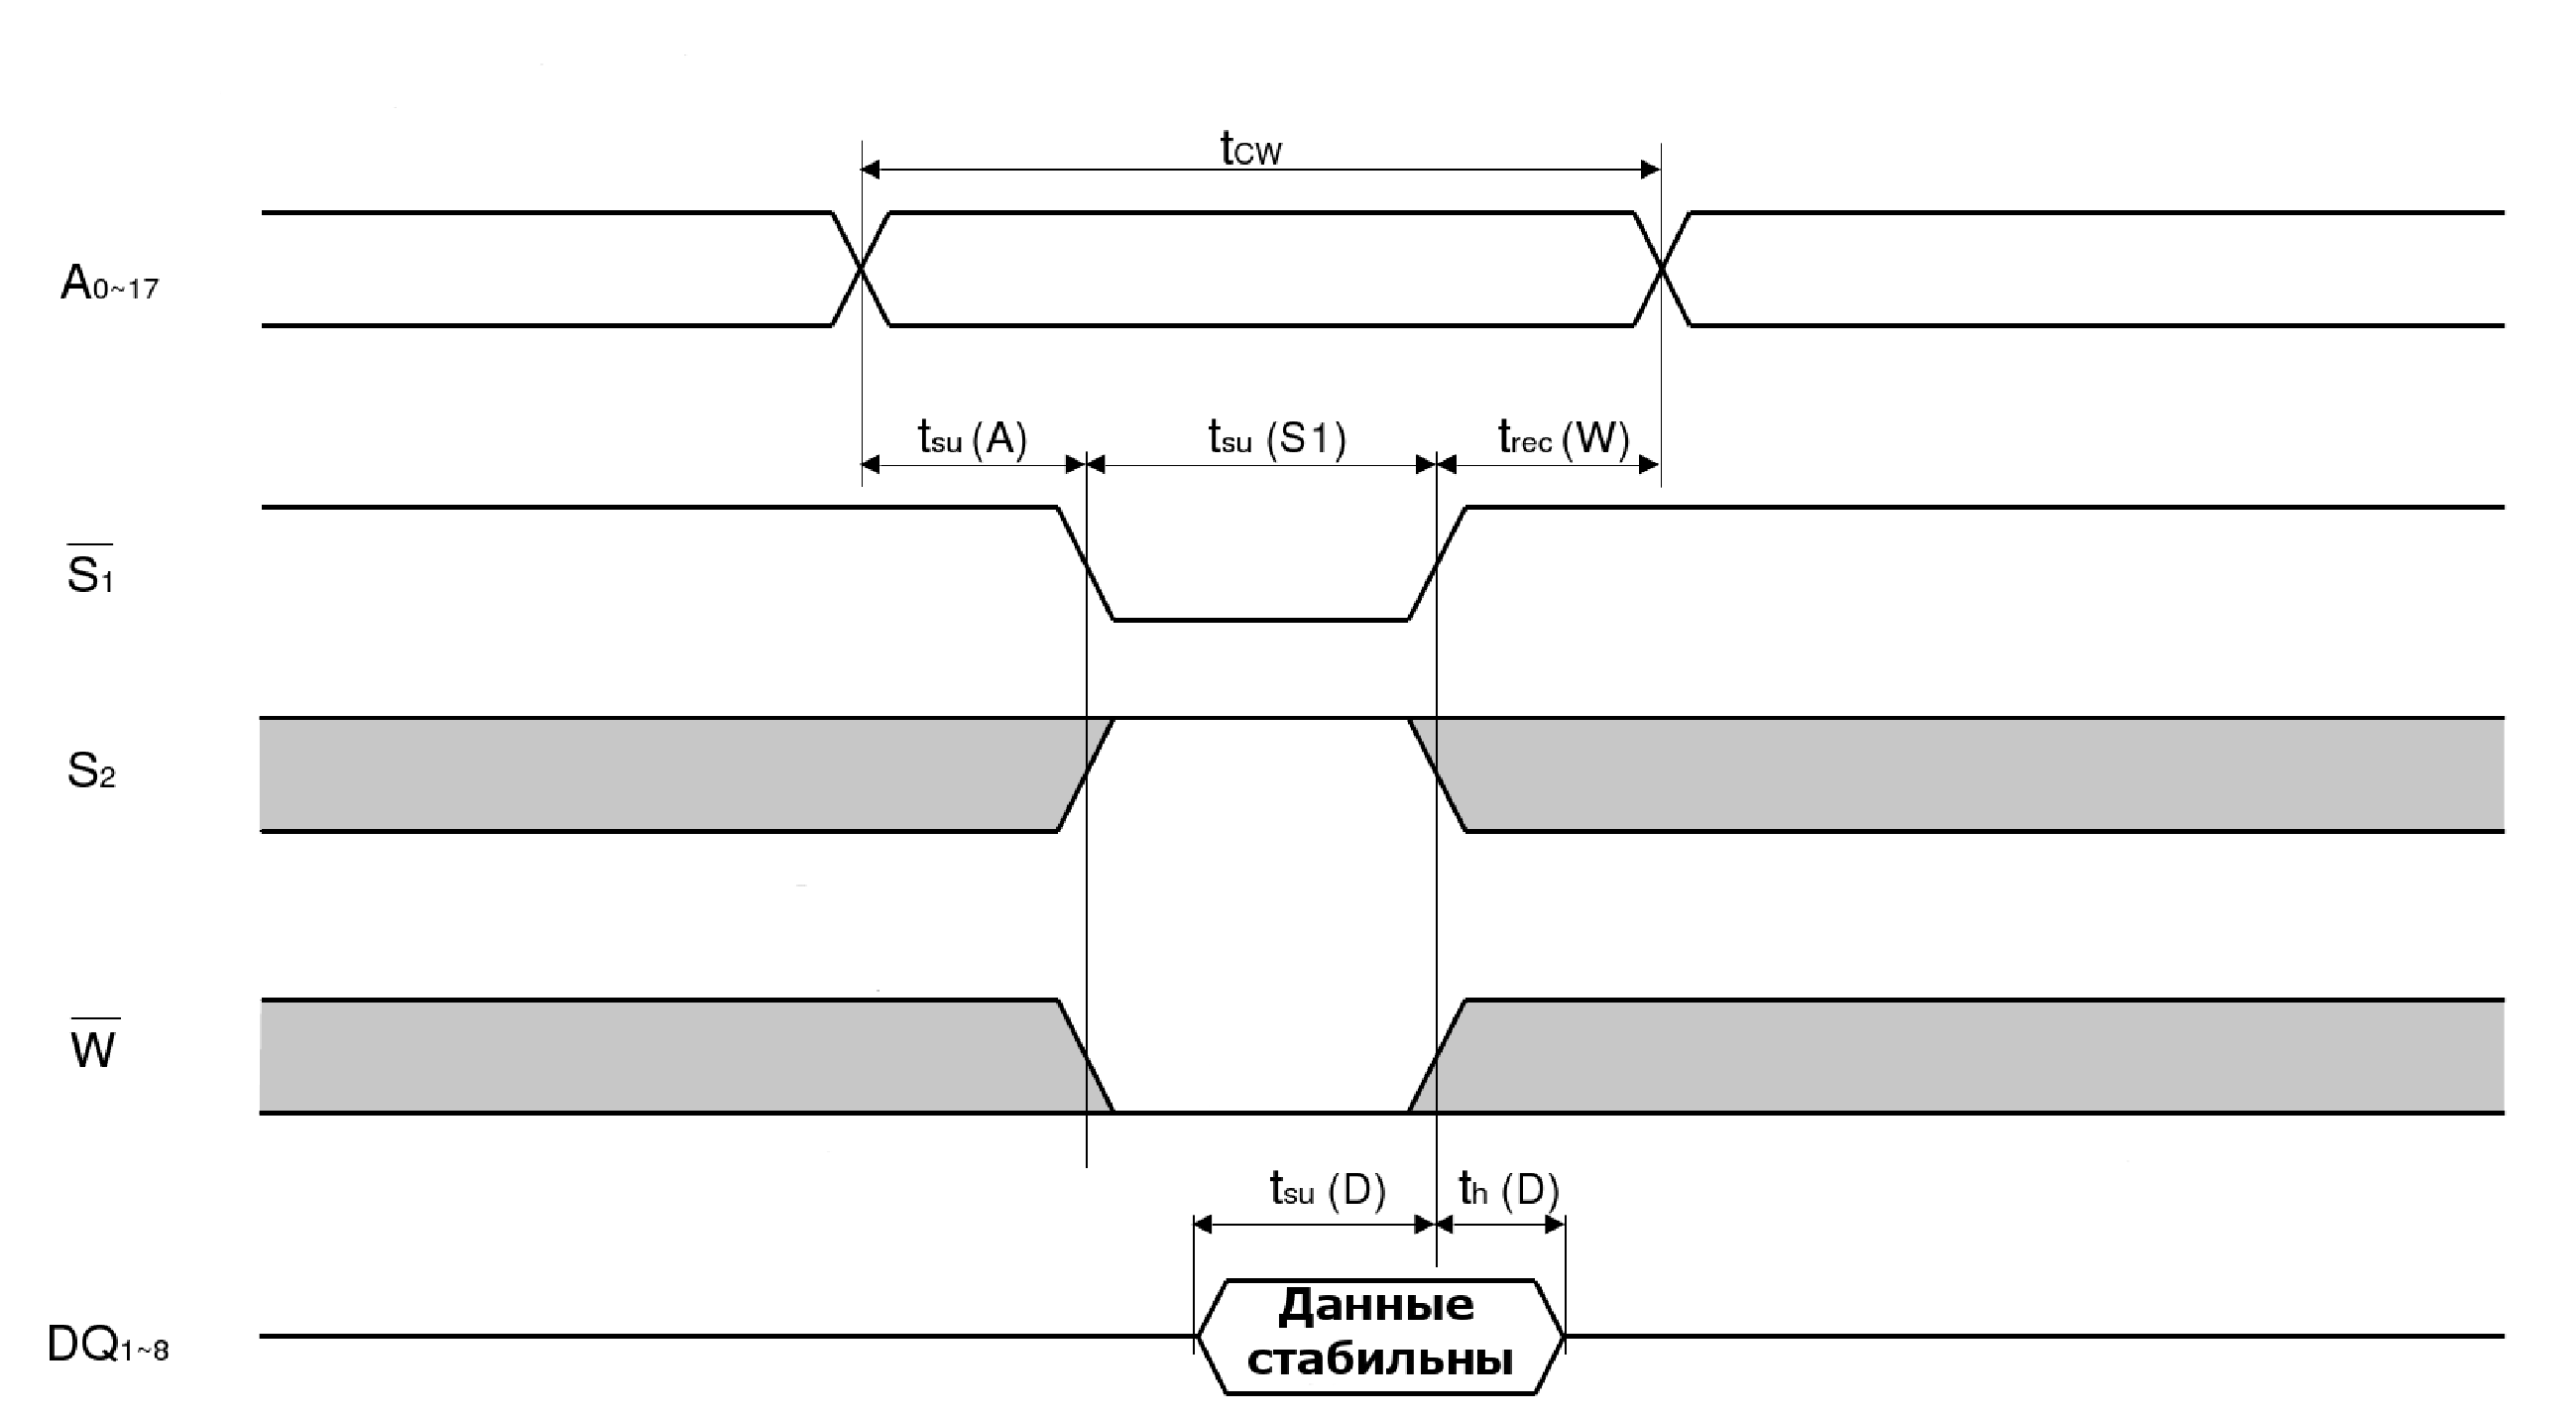
\includegraphics[width=1\linewidth]{./pics/sram_write_cycle.eps} }
\caption{Цикл записи}
\label{pic:sram_write_cycle}
\end{figure}

\begin{table}[H]
\begin{center}
\caption{Цикл операции записи в SRAM}
\label{tab:sram_write_cycle}
\begin{tabular}{|c|c|c|c|}
	\hline
		Название цикла & Обозначение & Время & Единицы \\
	\hline
		${t_{cw}}$ & Время цикла записи & 85 & ns \\
	\hline
		${t_w(W)}$ & Вркмя пульса записи & 60 & ns \\
	\hline
		${t_{su}(A)}$ & Время установки адреса & 0 & ns \\
	\hline
		${t_{su}(A-WH)}$ & Время установки адреса в соотв. с $\bar{E}$ & 70 & ns \\
	\hline
		${t_{su}(S_1)}$ & Время установки Chip Select 1 & 70 & ns \\
	\hline
		${t_{su}(S_2)}$ & Время установки Chip Select 1 & 70 & ns \\
	\hline
		${t_{su}(D)}$ & Время установки данных & 35 & ns \\
	\hline
		${t_{h}(D)}$ & Время удержания данных & 0 & ns \\
	\hline
		${t_{rec}(W)}$ & Время восстановления & 0 & ns \\
	\hline
		${t_{dis}(W)}$ & Время перехода после $\bar{W}$ низкого & 30 & ns \\
	\hline
		${t_{dis}(OE)}$ & Время перехода после $\bar{OE}$ высокого & 30 & ns \\
	\hline
		${t_{en}(W)}$ & Время перехода после $\bar{W}$ высокого & 30 & ns \\
	\hline
		${t_{en}(OE)}$ & Время перехода после $\bar{OE}$ низкого & 30 & ns \\
	\hline
\end{tabular}
\end{center}
\end{table}

Цикл чтения выполняется при высоком уровне сигнала $\bar{W}$ и низком уровне сигнала OE. В то же время сигналы
$\bar{S_1}$ и ${S_2}$ должны находится в активном состоянии. Подробнее последовательность действий отражена на
Рис.~\ref{pic:sram_read_cycle} и Таблице~\ref{tab:sram_read_cycle}.
Техническая реализация рассмотрена в разделе~\ref{sec:sram_controller} \\

\begin{figure}[H]
\center{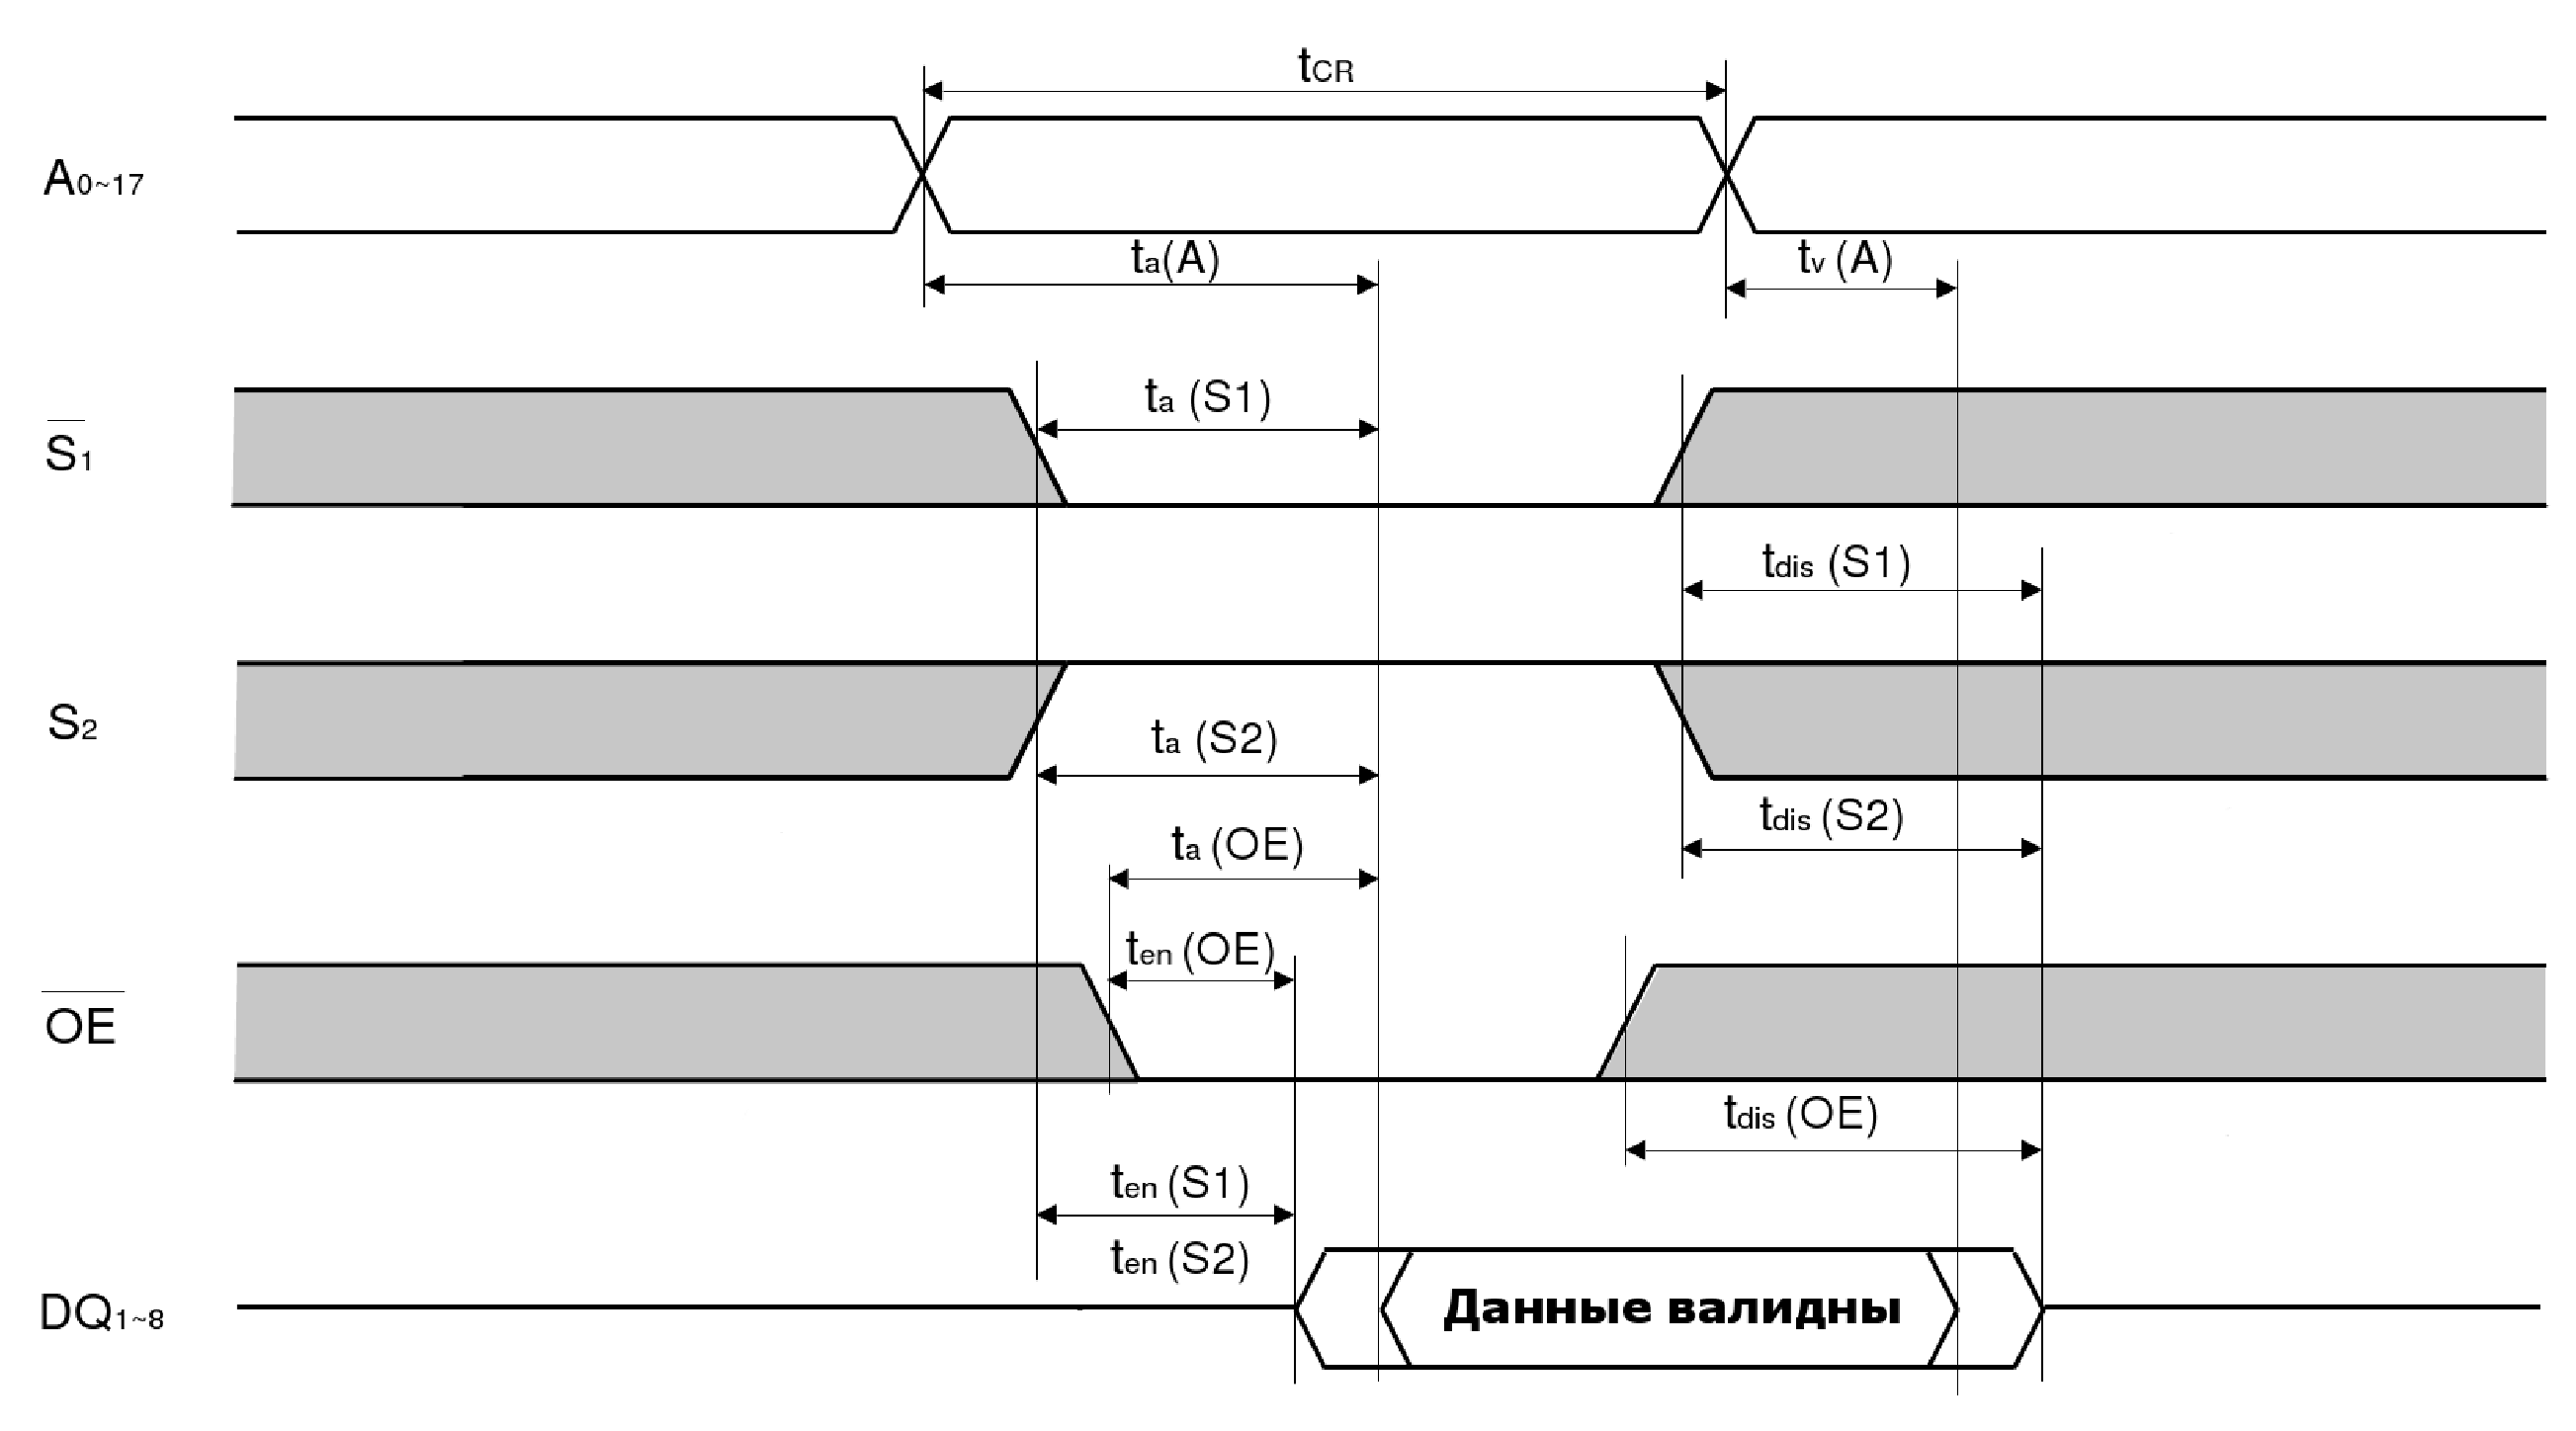
\includegraphics[width=1\linewidth]{./pics/sram_read_cycle.eps}}
\caption{Цикл чтения}
\label{pic:sram_read_cycle}
\end{figure}

\begin{table}[H]
\begin{center}
\caption{Цикл операции чтения из SRAM}
\label{tab:sram_read_cycle}
\begin{tabular}{|c|c|c|c|}
	\hline
		Название цикла & Обозначение & Время & Единицы \\
	\hline
		${t_{cr}(A)}$ & Время цикла чтения & 85 & ns \\
	\hline
		${t_a(A)}$ & Время доступа к адресу & 85 & ns \\
	\hline
		${t_a(S_1)}$ & Chip Select 1 & 85 & ns \\
	\hline
		${t_a(S_1)}$ & Chip Select 2 & 85 & ns \\
	\hline
		${t_a(OE)}$ & Время доступа к активному уровню OE & 45 & ns \\
	\hline
		${t_{dis}(S_1)}$ & Время перехода к низкому уровню & 30 & ns \\
	\hline
		${t_{dis}(S_2)}$ & Время перехода к низкому уровню & 30 & ns \\
	\hline
		${t_{dis}(OE)}$ & Время перехода после $\bar{OE}$ высокого уровня & 30 & ns \\
	\hline
		${t_{en}(S_1)}$ & Переход к активному состоянию для $\bar{S_1}$ & 10 & ns \\
	\hline
		${t_{en}(S_1)}$ & Переход к активному состоянию для ${S_2}$ & 10 & ns \\
	\hline
		${t_{en}(OE)}$ & Переход к активному состоянию для $\bar{OE}$ & 5 & ns \\
	\hline
		${t_{v}(A)}$ & Время валидности данных $\bar{OE}$ & 10 & ns \\
	\hline
\end{tabular}
\end{center}
\end{table}

Полное описание работы данной SRAM-микросхемы памяти приводится в описании на микросхему M5M5V208FP-85 \cite{sram}.

%--------------------------------------------------------------------------------
\subsection{Контроллер последовательного интерфейса для GPS микросхемы MAX2769}
Программирование режимов GPS микросхемы происходит через последовательный порт. Временные критерии и их значения
отражены на рисунке~\ref{pic:gps_serial} и таблице.~\ref{tab:gps_serial} соответственно. Техническая реализация приведена в
разделе ~\ref{razdel3_gps}.

\begin{figure}[h]
\center{\includegraphics[width=1\linewidth]{./pics/gps_serial_times.eps}}
\caption{Временная диарамма serial-интерфейса GPS}
\label{pic:gps_serial}
\end{figure}

\begin{table}[h]
\caption{Временные требования для serial-интерфейса}
\label{tab:gps_serial}
\begin{tabular}{|c|p{250pt}|c|p{70pt}|}
 \hline  
  Символ & Параметр & Значение & Единица измерения  \\  
 \hline  
  $t_{css}$  & Время между падающим фронтом сигнала $\bar {CS}$ и передним фронтом сигнала SCLK	& 10 & нс  \\  
 \hline  
  $t_{ds}$   & Время установки данных на serial-линию	& 10 & нс \\  
 \hline  
  $t_{dh}$   & Время удержания данных на serial-линии	& 10 & нс \\  
 \hline  
  $t_{ch}$   & Время нахождения Сlock-сигнала serial-интерфейса в состоянии 1 & 25 & нс \\  
 \hline  
  $t_{cl}$   & Время нахождения Сlock-сигнала serial-интерфейса в состоянии 0 & 25 & нс \\  
 \hline  
  $t_{csh}$  & Время между крайним возрастающим фронтом сигнала SCLK и падающим фронтом сигнала $\bar {CS}$ & 10 & нс \\  
 \hline  
  $t_{csw}$  & Время $\bar {CS}$ в активном состоянии    & 1 & такт \\  
 \hline  
\end{tabular}
\end{table}

Значения регистров можно найти в руководстве на микросхему MAX2769 \cite{gps_max}.
\newpage
					% специальный раздел 
%\section{ТЕХНОЛОГИЧЕСКИЙ РАЗДЕЛ}

\subsection{Описание аппаратной платформы для приема сигналов GPS}

\begin{figure}[H]
\center{\includegraphics[width=1\linewidth]{./pics/board_scheme.eps}}
\caption{Системы захвата данных}
\label{pic:board_scheme}
\end{figure}

\subsection{Описание разработанных встраиваемых решений (VHDL)}

% ===================== OLD =================================
\subsubsection{RS-232}
\label{razdel3_rs232}
Для реализации интерфейса RS232 

\subsubsection{Модули для SRAM-микросхемы M5M5V208FP-85}
\label{razdel3_sram}

\subsubsection{Модули для GPS микросхемы MAX2769}
\label{razdel3_gps}

\subsection{Контроллер для SRAM-микросхемы M5M5V208FP-85}
\label{sec:sram_controller}
%\begin{figure}[h]
%\center{\includegraphics[width=1\linewidth]{./pics/gps_serial_clock_oscylloscope.eps}}
%\caption{Clock-сигнал для serial-интерфейса GPS}
%\end{figure}

\subsection{Описание прикладного программного обеспечения}

\newpage
					% технологический раздел 
%\section*{Введение}
Целью данного дипломного проекта является разработка и реализация программно-аппаратных средств
для захвата и сопровождения сигнала спутниковой навигации. Оборудования захвата радиосигналов является очень востребованным.
На данный момент оно применяется в научных разработках посвещенных анализу и улучшению алгоритмов определения координат 
приемника сигналов, а так же в таких специфических исследованиях, как определение погоды по уровню сигнала спутников.
При разработке данного программного-аппаратного комплекса возникают различные вредные психофизиологические факторы, влияющие
на программиста, которые рассматриваются в разделе “Безопасность жизнедеятельности”.  

\newpage

\setcounter{section}{3}
\section{Безопасность жизнедеятельности}

\subsection{Анализ пожарной опасности в помещении небольших размеров, где установлена вычислительная техника}

Пожары в ВЦ представляют особую опасность, так как сопряжены с большими материальными потерями.
Характерная особенность ВЦ - небольшие площади помещений. Как известно пожар может возникнуть при взаимодействии
горючих веществ, окисления и источников зажигания. В помещениях ВЦ присутствуют все три основные фактора,
необходимые для возникновения пожара. Горючими компонентами на ВЦ являются: строительные материалы для
акустической и эстетической отделки помещений, перегородки, двери, полы, перфокарты и перфоленты, изоляция кабелей и др.

Противопожарная защита - это комплекс организационных и технических мероприятий, направленных на обеспечение безопасности людей,
на предотвращение пожара, ограничение его распространения, а также на создание условий для успешного тушения пожара.

Источниками зажигания в ВЦ могут быть электронные схемы от ЭВМ, приборы, применяемые для технического обслуживания,
устройства электропитания, кондиционирования воздуха, где в результате различных нарушений образуются перегретые элементы,
электрические искры и дуги, способные вызвать загорания горючих материалов.

В современных ЭВМ очень высокая плотность размещения элементов электронных схем. В непосредственной близости
друг от друга располагаются соединительные провода, кабели. При протекании по ним электрического тока выделяется
значительное количество теплоты. При этом возможно оплавление изоляции. Для отвода избыточной теплоты от ЭВМ служа
системы вентиляции и кондиционирования воздуха. При постоянном действии эти системы представляют собой дополнительную
пожарную опасность. Энергоснабжение ВЦ осуществляется от трансформаторной станции и двигатель-генераторных агрегатов.
На трасформаторных подстанциях особую опасность представляют трансформаторы с масляным охлаждением. В связи с этим
предпочтение следует отдавать сухим транформатором. Пожарная опасность двигатель-генераторных агрегатов обусловленна
возможностью коротких замыканий, перегрузки, электрического искрения. Для безопасной работы необходим правильный
расчет и выбор аппаратов защиты. При поведении обслуживающих, ремонтных и профилактических работ используются
различные смазочные вещества, легковоспламеняющиеся жидкости, прокладываются временные электропроводники, ведут пайку
и чистку отдельных узлов. Возникает дополнительная пожарная опасность, требующая дополнительных мер пожарной защиты.
В частности, при работе с паяльником следует использовать несгораемую подставку с несложными приспособлениями
для уменьшения потребляемой мощности в нерабочем состоянии.

Для большинства помещений ВЦ установлена категория пожарной опасности В \cite{npb10503}. Одной из наиболее важных задач пожарной защиты
является защита строительных помещений от разрушений и обеспечение их достаточной прочности в условиях воздействия
высоких температур при пожаре. Учитывая высокую стоимость электронного оборудования ВЦ, а также категорию его
пожарной опасности, здания для ВЦ и части здания другого назначения, в которых предусмотрено размещение ЭВМ должны
быть 1 и 2 степени огнестойкости. Для изготовления строительных конструкций используются, как правило, кирпич,
железобетон, стекло, металл и другие негорючие материалы. Применение дерева должно быть ограниченно, а в
случае использования необходимо пропитывать его огнезащитными составами. В ВЦ противопожарные преграды в виде
перегородок из несгораемых материалов устанавливают между машинными залами.

\subsection{Оснащение помещения устойством для локального тушения пожаров}

К средствам тушения пожара, предназначенных для локализации небольших загораний, относятся пожарные стволы,
внутренние пожарные водопроводы, огнетушители, сухой песок, асбестовые одеяла и т. п. В зданиях ВЦ пожарные
краны устанавливаются в коридорах, на площадках лестничных клеток и входов. Вода используется для тушения пожаров
в помещениях программистов, библиотеках, вспомогательных и служебных помещениях. Применение воды в машинных залах
ЭВМ, хранилищах носителей информации, помещениях контрольно измерительных приборов ввиду опасности повреждения или
полного выхода из строя дорогостоящего оборудования возможно в исключительных случаях, когда пожар принимает
угрожающе крупные размеры. При этом количество воды должно быть минимальным, а устройства ЭВМ необходимо защитить
от попадания воды, накрывая их бризентом или полотном.

Для тушения пожаров на начальных стадиях широко применяются огнетушители. По виду используемого огнетушащего
вешества огнетушители подразделяются на следующие основные группы. Пенные огнетушители, применяются для тушения
горящих жидкостей, различных материалов, конструктивных элементов и оборудования, кроме электрооборудования,
находящегося под напряжением. Газовые огнетушители применяются для тушения жидких и твердых веществ, а также
электроустановок, находящихся под напряжением. В производственных помещениях ВЦ применяются главным образом
углекислотные огнетушители, достоинством которых является высокая эффективность тушения пожара, сохранность
электронного оборудования, диэлектрические свойства углекислого газа, что позволяет использовать эти огнетушители
даже в том случае, когда не удается обесточить электроустановку сразу. Для обнаружения начальной стадии
загорания и оповещения службу пожарной охраны используют системы автоматической пожарной сигнализации (АПС).
Кроме того, они могут самостоятельно приводить в действие установки пожаротушения, когда пожар еще не достиг
больших размеров. Системы АПС состоят из пожарных извещателей, линий связи и приемных пультов (станций).
Эффективность применения систем АПС определяется правильным выбором типа извещателей и мест их установки.
При выборе пожарных извещателей необходимо учитывать конкретные условия их эксплуатации: особенности помещения и
воздушной среды, наличие пожарных материалов, характер возможного горения, специфику технологического процесса и т.п.

Особое внимание уделяется пожарной безопасности, так как пожары в ВЦ сопряжены с опасностью для человеческой
жизни и большими материальными потерями.

В соответствии с "Типовыми правилами пожарной безопасности для промышленных предприятий" залы ЭВМ, помещения
для внешних запоминающих устройств, подготовки данных, сервисной аппаратуры, архивов, копировально множительного
оборудования и т.п. необходимо оборудовать дымовыми пожарными извещателями. В этих помещениях в начале пожара
при горении различных пластмассовых, изоляционных материалов и бумажных изделий выделяется значительное количество
дыма и мало теплоты. В других помещениях ВЦ, в том числе в машинных залах дизель генераторов и лифтов, трансформаторных
и кабельных каналах, воздуховодах допускается применение тепловых пожарных извещателей. Объекты ВЦ кроме АПС необходимо
оборудовать установками стационарного автоматического пожаротушения. Наиболее целесообразно применять в ВЦ установки
газового тушения пожара, действие которых основано на быстром заполнении помещения огнетушащим газовым веществом с
резким смижением содержания в воздухе кислорода.

Меры по пожарной профилактики:
\begin{itemize}
\item строительно-планировочные;
\item технические;
\item способы и средства тушения пожаров;
\item организационные.
\end{itemize}

Строительно-планировочные определяются огнестойкостью зданий и сооружений (выбор материалов конструкций: сгораемые, несгораемые,
трудносгораемые) и предел огнестойкости — это количество времени, в течение которого под воздействием огня не нарушается
несущая способность строительных конструкций вплоть до появления первой трещины.

Все строительные конструкции по пределу огнестойкости подразделяются на 8 степеней от 1/7 ч до 2ч.

Для помещений ВЦ используются материалы с пределом стойкости от 1-5 степеней. В зависимости от степени огнестойкости определены
наибольшие дополнительные расстояния от выходов для эвакуации при пожарах (5 степень — 50 м).

Технические меры:
\begin{itemize}
\item это соблюдение противопожарных норм при эвакуации систем вентиляции, отопления, освещения, эл. обеспечения и т.д.
\item использование разнообразных защитных систем;
\item соблюдение параметров технологических процессов и режимов работы оборудования.
\end{itemize}

Организационные меры — проведение обучения по пожарной безопасности, соблюдение мер по пожарной безопасности.

Средства пожаротушения:
\begin{description}
\item[a)]Ручные
	\begin{itemize}
	\item огнетушитель порошковый;
	\item огнетушитель углекислотный, бромэтиловый
	\end{itemize}

\item[б)] Cистема пожаротушения ручного действия (кнопочный извещатель).
Для ВЦ используются тепловые датчики-извещатели типа ДТЛ, дымовые радиоизотопные типа РИД.
\end{description}

Для ВЦ используются огнетушители углекислотные ОУ, ОА (создают струю распыленного бром этила).

Способ соединения датчиков в системе эл. пожарной сигнализации с приемной станцией может быть — параллельным (лучевым);
— последовательным (шлейфным).

Норма оснащения помещения категории В  переносными огнетушителями составляет(предельная защищаемая площадь 200м$^2$) 
\cite{bjd421}:
\begin{description}

	\item[a)] порошковые огнетушители:
		\begin{itemize}
		\item 2 огнетушителя весом 2кг для категории пожаров A, B, C, D, E;
		\item 1 огнетушитель весом 8кг для категории пожаров A, B, C, D, E;
		\end{itemize}
	\item[б)] 	углекислотные огнетушители:
		\begin{itemize}
		\item 2 огнетушителя весом 3кг для категории пожаров E;
		\end{itemize}

\end{description}

\subsection{Экологическая оценка проектируемой компьютерной техники}
Внедрение в промышленность новых, более эффективных промышленных процессов, резкое повышение продуктивности и расширение
масштабов производства потребовали увеличения затрат материальных и энергетических ресурсов, что, в свою очередь,
привело к росту отрицательного воздействия на окружающую среду. Основными проблемами по решению задач защиты окружающей
среды являются: совершенствование технологических процессов и разработка нового оборудования с меньшим уровнем выброса
примесей и отходов в окружающую среду, также необходимо уменьшить влияние таких факторов как шум при работе, излучение
высокочастотных электромагнитных полей, сильный разогрев и т.п.

Более 80\% общей трудоемкости производства вычислительной техники связано с производством печатных плат.
При изготовлении печатных плат происходит загрязнение воздушного пространства парами свинца \cite{bjd43}, а соединения кислот и
щелочей загрязняют сточные воды предприятия. При производстве плат должны предусматриваться эффективные средства
защиты окружающей среды от возможного загрязнения.

Лидер в области бессвинцового производства – японская промышленность. Начало его организации было положено в декабре 1997 года
после издания закона о контроле утилизации веществ, содержащих свинец. Их подлежало герметично упаковывать перед захоронением
для предотвращения выщелачивания свинца на поверхность.

В апреле 1998 года Япония начала реализацию проекта по изучению бессвинцового процесса, названного NEDO, целью которого было
создание базы данных по бессвинцовым припоям для удобства выбора материала и разработки технологии пайки.
Общий бюджет проекта составил 350 млн. иен за два года. Участники проекта – представители крупнейших японских
производителей электронных систем, компонентов и сплавов. В результате уже к 2001 году следующие крупнейшие японские
производители сумели сформировать собственные планы полного отказа от свинцовой пайки:
\begin{itemize}
\item Matsushita (Panasonic) еще в октябре 1998 года выпустила первый компактный мини-дисковый плеер, выполненный с
	использованием только бессвинцового сплава Sn/Ag/Bi/Cu. К 2001 году компания провозгласила полный отказ от применения свинца;
\item Sony в 2001 году полностью исключила применение свинца при монтаже устройств с повышенной плотностью;
\item Toshiba к 2000 году прекратила использовать свинец при производстве мобильных телефонов;
\item Hitachi к 1999 году сократила использование свинца на 50\% по сравнению с 1997-м. К 2001-му вся продукция компании
	выпускалась уже без применения свинца.
\end{itemize}

Гальванические работы сопряжены с использованием больших объёмов воды для приготовления растворов электролитов и
промывочных операций. Поэтому сточные воды в этих случаях значительно загрязнены ядовитыми химическими веществами.
Кроме того, воздух, удаляемый от технологического гальванического оборудования, содержит большое количество вредных
веществ в различных агрегатных состояниях: капель жидком, паро- и газообразном.Технологические процессы сварки и
пайки сопровождаются выделением пыли и токсичных газов, а сточные воды могут загрязняться механическими примесями,
кислотами. Процесс получения функционально завершённого изделия заканчивается сборочными операциями. Отрицательное
воздействие на окружающую среду процессов сборки менее ощутимо. Однако и в этих случаях при проведении
санитарно-гигиенической обработки производственных помещений в сточные воды могут попадать различные нежелательные примеси.

В настоящее время широко используются пассивные методы защиты, суть которых сводится к ограничению количества
загрязняющих окружающую среду выбросов, т.е. улавливанию пылегазовыделений, выбрасываемых в атмосферу, очистка
сточных вод от примесей и т.п. При производстве модулей должны использоваться пассивные фильтры, которые основаны
на способности пористых материалов задерживать частицы примесей при движении дисперсных сред. Частицы примесей оседают
на входной части фильтроэлемента, помещённого в корпус. Осаждение частиц происходит в результате совокупного действия
эффекта касания, диффузионных, инерционных гравитационных процессов. Для очистки воздуха от туманов кислот, щелочей,
масел и других жидкостей используются волоконные фильтры, принцип действия которых основан на осаждении капель на
поверхности материалов и последующего отекания жидкостей под воздействием сил тяжести.

При загрязнении сточных вод маслосодержащим и примесями, помимо отстаивания и фильтрования, применяется также
процесс флотации. Очистка вод флотацией заключается в интенсификации процесса маслопродуктов при их частиц
пузырьками воздуха, попадающего в сточную воду. Таким образом, наиболее перспективной формой защиты окружающей
среды от вредного воздействия является «безотходная» технология и комплекс природоохранных мероприятий в
технологических процессах от обработки сырья до использования готовой продукции.

\newpage

\section*{Заключение}
В разделе "Безопасность жизнедеятельности" был проведен анализ пожарной опасности в помещении небольших размеров,
где установлена ВТ. Разработаны мероприятия по оснащению помещения устройством для локального тушения пожаров. Дана
экологическая оценка проектируемой компьютерной техники.

\newpage
					% архиважно биля 
%\section{ОРГАНИЗАЦИОННО-ЭКОНОМИЧЕСКИЙ РАЗДЕЛ}
\subsection{Планирование разработки программных средств с построением графика}
Целью дипломного проекта является разработка программно-аппаратного комплекса (ПК) захвата GNSS сигналов.
В данном разделе определяется трудоёмкость и затраты на создание ПК, а так же производится расчёт основных технико-экономических
показателей проекта.

\subsubsection*{Определение трудоемкости и продолжительности работ по созданию ПК}
Процесс разработки включает: обзор и анализ программных средств схожей тематики, анализ и выбор программных продуктов для
создания программы; отладка; испытание. В свою очередь каждый из этих этапов можно подразделить на отдельные под этапы.
Согласно ГОСТ 23501.1-79 регламентируются следующие стадии проведения исследования:

\begin{itemize}
	\item техническое задание – ТЗ (ГОСТ 23501.2-79);
	\item эскизный проект – ЭП (ГОСТ 23501.5-80);
	\item технический проект – ТП (ГОСТ 23501.6-80);
	\item рабочий проект – РП (ГОСТ 23501.11-81);
	\item внедрение – ВП (ГОСТ 23501.15-81).
\end{itemize}

Планирование стадий и содержания работ осуществляется в соответствии с \cite{bibl51}. На всех стадиях проведения исследования
выполняются следующие виды работ, перечень которых показан в таблице ~\ref{tab:eco1}.

% http://users.sdsc.edu/~ssmallen/latex/longtable.html
\begin{center}
\begin{longtable}{|l|l|}
\caption{Состав работ и стадии разработки ПК} \label{tab:eco1} \\ \hline
\multicolumn{1}{|c|}{\textbf{Стадии разработки}}    &   \multicolumn{1}{c|}{\textbf{Перечень работ}} \\ \hline
\multicolumn{1}{|c|}{\textbf{1}}    &   \multicolumn{1}{|c|}{\textbf{2}} \\ \hline
\endfirsthead

%\multicolumn{2}{c} %
%{{\bfseries \tablename \thetable{} -- continued from previous page}} \\
\multicolumn{2}{|l|}{{Продолжение таблицы ~\ref{tab:eco1}}} \\ %\hline
\hline \multicolumn{1}{|c|}{\textbf{1}} &
%\multicolumn{1}{c|}{\textbf{Triple chosen}} &
\multicolumn{1}{c|}{\textbf{2}} \\ \hline 
\endhead

%\multicolumn{2}{|r|}{{}} \\ %\hline
%\hline \multicolumn{2}{|r|}{{Continued on next page}} \\ %\hline
\endfoot

\hline
\endlastfoot
\\
		Техническое задание & \begin{parbox}{5in} {
						\begin{itemize}
							\item постановка задачи;
							\item подбор литературы;
							\item сбор исходных данных;
							\item определение требований к системе;
							\item определение стадий, этапов и сроков разработки ПК;
						\end{itemize} }  
					\end{parbox} \\
	\hline
		Эскизный проект & \begin{parbox}{5in} {
					\begin{itemize} 
						\item анализ программных средств схожей тематики;
						\item разработка общей структуры ПК;
						\item разработка структуры программы по подсистемам;
						\item документирование;
					\end{itemize} }
				\end{parbox} \\
	\hline
		Технический проект & \begin{parbox}{5in} {
					\begin{itemize} 
						\item определение требований к ПК;
						\item выбор инструментальных средств;
						\item определение свойств и требований к аппаратному обеспечению;
					\end{itemize} } 
				\end{parbox} \\
	\hline
		Рабочий проект & \begin{parbox}{5in} {
					\begin{itemize} 
						\item программирование;
						\item тестирование и отладка ПК;
						\item разработка программной документации;
						\item согласование и утверждение программы и методики испытаний;
					\end{itemize} }
				\end{parbox} \\
	\hline
		Внедрение & \begin{parbox}{5in} {
					\begin{itemize}
						\item опытная эксплуатация;
						\itemнализ данных полученных в результате эксплуатации;
						\item корректировка технической документации по результатам испытаний;
					\end{itemize} }
				\end{parbox} \\
\end{longtable}
\end{center}

Трудоемкость разработки ПК определяется по сумме трудоемкости этапов и видов работ, оцениваемых экспертным путем в
человеко-днях, и носит вероятностный характер, так как зависит от множества трудно учитываемых факторов.

Трудоемкость каждого вида работ определяется в соответствии с методическими указаниями \cite{bibl53} по формуле:

\begin{equation}
t_i = \frac{3\cdot{t_{min}} + 2\cdot{t_{max}}}{5},
\label{eq:eco1}
\end{equation}
где:	$t_{min}$ - минимально возможная трудоемкость выполнения отдельного вида работ в человеко-днях; \\
	$t_{max}$ - максимально возможная трудоемкость выполнения отдельного вида работ в человеко-днях.

Продолжительность каждого вида работ в календарных днях ${(T_i)}$ определяется по формуле \cite{bibl53}:

\begin{equation}
T_i = \frac{t_i}{\mbox{Ч}_i}\cdot{K_{\mbox{вых}}},
\label{eq:eco2}
\end{equation}
где:	${t_i}$ - трудоемкость работы, человек-дней; \\
	${\mbox{Ч}_i}$ - численность исполнителей, человек; \\
	${K_{\mbox{вых}}}$ - коэффициент, учитывающий выходные и праздничные дни: \\

\begin{equation}
T_i = \frac{K_{\mbox{кап}}}{K_{\mbox{раб}}},
\label{eq:eco3}
\end{equation}
где:	${K_{\mbox{кап}}}$ - число календарных дней;
	${K_{\mbox{раб}}}$ - рабочие дни.

Для расчёта принимается среднее значение ${K_{\mbox{вых}} = 1.45}$. 

Полный список видов и этапов работ по созданию ПС, экспертные оценки и расчетные величины их трудоемкости,
а также продолжительность каждого вида работ, рассчитанные по формулам (\ref{eq:eco1}) и (\ref{eq:eco2}) представлены
в таблице ~\ref{tab:eco2}.

\begin{center}
\begin{longtable}{|c|p{3.5cm}|c|c|c|c|c|}
\caption{Расчёт трудоёмкости и продолжительности работ по созданию ПК} \label{tab:eco2} \\ \hline
\multicolumn{1}{|c|}{\textbf{№}} & \multicolumn{1}{p{3.5cm}|}{\textbf{Наименование стадий и  работ}} & 
\multicolumn{3}{p{3.5cm}|}{\textbf{Трудоемкость, человеко-дни}} &   \multicolumn{1}{p{3cm}|}{\textbf{Кол-во исполнителей, чел.}} &
\multicolumn{1}{p{3.8cm}|}{\textbf{Продолжитель-ность, календарные дни}} \\
\cline{3-7}

\multicolumn{1}{|c|}{} &   \multicolumn{1}{c|}{} & 
\multicolumn{1}{|c|}{${t_{min}}$} & \multicolumn{1}{c|}{${t_{max}}$} & 
\multicolumn{1}{|c|}{ ${t_i}$ } &   \multicolumn{1}{c|}{ ${\mbox{Ч}_i}$ } & 
\multicolumn{1}{c|}{ ${T_i}$ } \\ \hline

\multicolumn{1}{|c|}{\textbf{1}} &   \multicolumn{1}{c|}{\textbf{2}} & 
\multicolumn{1}{|c|}{\textbf{3}} &   \multicolumn{1}{c|}{\textbf{4}} & 
\multicolumn{1}{|c|}{\textbf{5}} &   \multicolumn{1}{c|}{\textbf{6}} & 
\multicolumn{1}{c|}{\textbf{7}} \\ \hline
\endfirsthead

\multicolumn{7}{|l|}{{Продолжение таблицы ~\ref{tab:eco2}}} \\ %\hline
\hline
\multicolumn{1}{|c|}{\textbf{1}} &   \multicolumn{1}{c|}{\textbf{2}} & 
\multicolumn{1}{c|}{\textbf{3}} & \multicolumn{1}{c|}{\textbf{4}} & 
\multicolumn{1}{|c|}{\textbf{5}} &   \multicolumn{1}{c|}{\textbf{6}} & 
\multicolumn{1}{c|}{\textbf{7}} \\ \hline
\endhead

\endfoot

\hline
\endlastfoot

\multicolumn{7}{|c|}{\textbf{Техническое задание}} \\ \hline

1. & Постановка задачи & & & & &\\ \hline
2. & Подбор литературы & & & & &\\ \hline
3. & Сбор исходных данных & & & & &\\ \hline
4. & Определение требований к системе & & & & &
	\\ \hline
5. & Определение ста-дий, этапов и сроков разработки ПК
	& & & & & \\ \hline

\multicolumn{7}{|c|}{\textbf{Эскизный проект}} \\ \hline

6. & Анализ программных средств схожей тематики & & & & &\\ \hline
7. & Разработка общей структуры ПК & & & & &\\ \hline
8. & Разработка структуры программы по подсистемам & & & & &\\ \hline
9. & \hfill{}Документирование & & & & & \\ \hline

\multicolumn{7}{|c|}{\textbf{Технический проект}} \\ \hline

10. & Определение требований к ПК & & & & &\\ \hline
11. & Выбор языка программирования & & & & &\\ \hline
12. & Определение свойств и требований к аппаратному обеспечению & & & & &\\ \hline

\multicolumn{7}{|c|}{\textbf{Рабочий проект}} \\ \hline

13. & Дизайн проекта & & & & &\\ \hline
14. & \hfill{}Программирование & & & & &\\ \hline
15. & Тестирование и отладка ПК & & & & &\\ \hline
16. & Разработка программной документации & & & & & \\ \hline
17. & Согласование и утверждение программы и методики испытаний & & & & & \\ \hline

\multicolumn{7}{|c|}{\textbf{Внедрение}} \\ \hline

18. & Опытная эксплуатация & & & & &\\ \hline
19. & Анализ данных полученных в результате эксплуатации & & & & &\\ \hline
20. & Корректировка технической документации по результатам испытаний & & & & &\\ \hline

    & Итого & & & XXX & & XXX \\ \hline

\hline
\end{longtable}
\end{center}

Таким образом, общая трудоёмкость разработки ПС составляет  88 человеко-дней, а их продолжительность – 112 календарных дней.

\subsubsection*{Построение ленточного графика разработки ПС}
В качестве инструмента планирования работ используем ленточный график. Ленточный график является удобным, простым и наглядным
инструментом для планирования работ. Он представляет собой таблицу, где перечислены  работы и длительность выполнения каждой
из них. Продолжением таблицы является линейный график, построенный в масштабе, наглядно показывающий продолжительность
каждой работы в виде отрезков прямых,  располагающихся в соответствии с последовательностью выполнения работ.

Ленточный график разработки ПС, построенный на основе данных табл. ~\ref{tab:eco2} приведён на рисунке ~\ref{pic:line_graphic} 
Он позволяет наглядно представить логическую последовательность и взаимосвязь отдельных работ, сроки начала и окончания работ,
соблюдение которых обеспечит своевременное выполнение проекта и разработку программных средств.

% Picture here

\subsection{Расчет сметы затрат на  разработку ПС}
Сметная стоимость проектирования и внедрения программы включает в себя  затраты, определяемые по формуле (\ref{eq:eco_smeta}):

\begin{equation}
C_{\mbox{пр}} = C_{\mbox{осн}} + C_{\mbox{доп}} + C_{\mbox{соц}} + C_{\mbox{м}} + C_{\mbox{маш.вр.}} + C_{\mbox{н}},
\label{eq:eco_smeta}
\end{equation}
где:	${C_{\mbox{пр}}}$ - стоимость разработки ПС; \\
	${C_{\mbox{м}}}$ - затраты на используемые материалы; \\
	${C_{\mbox{осн}}}$ - основная заработная плата исполнителей; \\
	${C_{\mbox{доп}}}$ - дополнительная заработная плата исполнителей, учитывающая потери времени на отпуска и болезни
		(принимается в среднем 10\% от основной заработной платы); \\
	${C_{\mbox{соц}}}$ - единый социальный налог (ЕСН), представляющий собой отчисления во внебюджетные фонды
		государственного социального страхования (пенсионный фонд, фонд обязательного медицинского страхования,
		фонд социального страхования). Рассчитывается в соответствии с установленной ставкой ЕСН как 26\% от
		основной и дополнительной заработной платы; \\
	${C_{\mbox{н}}}$ - накладные расходы включают затраты на управление, уборку, ремонт, электроэнергию, отопление и
		другие хозяйственные расходы (принимаются в размере 60\% от основной и дополнительной заработной платы);
	${C_{\mbox{маш.вр.}}}$ - стоимость машинного времени. \\

\subsubsection*{Основная заработная плата исполнителей}
На статью «Заработная плата» относят заработную плату научных, инженерно-технических и других работников,
непосредственно участвующих в разработке ПС. Расчёт ведётся по формуле (\ref{eq:eco_zarplata}):
\begin{equation}
\mbox{З}_{\mbox{исп}} = \mbox{З}_{\mbox{ср}} \cdot{T},
\label{eq:eco_zarplata}
\end{equation}
где:	${\mbox{З}_{\mbox{исп}}}$ - заработная плата исполнителей (руб.); \\
	${\mbox{З}_{\mbox{ср}}}$ -  средняя дневная тарифная ставка работника организации разработчика ПС (руб./чел.дни); \\
	${T}$ - трудоёмкость разработки ПС (чел.дни). \\

${\mbox{З}_{\mbox{ср}}}$ определяется по формуле (\ref{eq:eco_zsr}):
\begin{equation}
\mbox{З}_{\mbox{ср}} = \frac{C}{\mbox{Ф}_{\mbox{мес}}},
\label{eq:eco_zsr}
\end{equation}
где:	${C}$ - месячная зарплата работника (руб./мес.); \\
	${\mbox{Ф}_{\mbox{мес}}}$ - среднее количество рабочих дней в месяце (20дн.). \\

Расчёт затрат на основную заработную плату разработчиков ПС приведен в таблице \ref{tab:eco_zarplata}.

\begin{center}
\begin{longtable}{|c|c|c|c|c|c|}
\caption{Затраты на заработную плату} \label{tab:eco_zarplata} \\ \hline
\multicolumn{1}{|c|}{\textbf{№}} & \multicolumn{1}{c|}{\textbf{Исполнитель}} & 
\multicolumn{1}{p{2.5cm}|}{\textbf{Оклад, руб./мес.}} &   \multicolumn{1}{p{2.5cm}|}{\textbf{Оклад, руб./день}} & 
\multicolumn{1}{p{3.5cm}|}{\textbf{Трудоемкость, чел. дней}} & \multicolumn{1}{p{2cm}|}{\textbf{Сумма, руб.}} \\ \hline

\multicolumn{1}{|c|}{\textbf{1}} &   \multicolumn{1}{c|}{\textbf{2}} & 
\multicolumn{1}{c|}{\textbf{3}} &   \multicolumn{1}{c|}{\textbf{4}} & 
\multicolumn{1}{c|}{\textbf{5}} & \multicolumn{1}{c|}{\textbf{6}} \\ \hline
\endfirsthead

\multicolumn{6}{|l|}{{Продолжение таблицы ~\ref{tab:eco_zarplata}}} \\ %\hline
\hline
\multicolumn{1}{|c|}{\textbf{1}} &   \multicolumn{1}{c|}{\textbf{2}} & 
\multicolumn{1}{c|}{\textbf{3}} &   \multicolumn{1}{c|}{\textbf{4}} & 
\multicolumn{1}{c|}{\textbf{5}} & \multicolumn{1}{c|}{\textbf{6}} \\ \hline
\endhead

\endfoot

\hline
\endlastfoot

1. & Руководитель & 40000 & 2000 & 5 & 10000 \\ \hline
2. & Инженер & 30000 & 1500 & 75 & 112500 \\ \hline
 & Итого ${C_{\mbox{осн}}}$ & - & - & 80 & 122500 \\

\hline

\end{longtable}
\end{center}

\subsubsection*{Дополнительная заработная плата}
Дополнительная заработная плата на период разработки ПС рассчитывается относительно основной и составляет 10\% от её величины:

\begin{equation}
C_{\mbox{доп}} = C_{\mbox{осн}} \cdot 0.1 = 122500 \cdot 0.1 = 12250,
%\label{eq:eco_smeta}
\end{equation}

\subsubsection*{Расчёт отчислений на социальное страхование}
Отчисления на социальное страхование рассчитываются относительно выплаченной заработной платы (суммы основной и
дополнительной заработной платы). Составляют 26\%:

\begin{equation}
C_{\mbox{соц}} = (C_{\mbox{доп}} + C_{\mbox{осн}}) \cdot 0.26 = (122500 + 12250) \cdot 0.26 = 35035 (\mbox{руб}),
%\label{eq:eco_smeta}
\end{equation}

\subsubsection*{Расчёт расходов на материалы}
На эту статью относят все затраты на магнитные носители данных, бумагу, для печатных устройств, канцтовары и др.
Затраты по ним определяются по экспертным оценкам. Расчёт расходов на материалы приведён в табл. \ref{tab:eco_zatnm}

\begin{center}
\begin{longtable}{|c|c|c|c|}
\caption{Затраты на заработную плату} \label{tab:eco_zatnm} \\ \hline
\multicolumn{1}{|c|}{\textbf{№}} & \multicolumn{1}{c|}{\textbf{Материалы}} & 
\multicolumn{1}{c|}{\textbf{Кол-во, шт}} &   \multicolumn{1}{c|}{\textbf{Стоимость, руб.}} \\ \hline

\multicolumn{1}{|c|}{\textbf{1}} &   \multicolumn{1}{c|}{\textbf{2}} & 
\multicolumn{1}{c|}{\textbf{3}} &   \multicolumn{1}{c|}{\textbf{4}} \\ \hline
\endfirsthead

\multicolumn{4}{|l|}{{Продолжение таблицы ~\ref{tab:eco_zatnm}}} \\ %\hline
\hline
\multicolumn{1}{|c|}{\textbf{1}} &   \multicolumn{1}{c|}{\textbf{2}} & 
\multicolumn{1}{c|}{\textbf{3}} &   \multicolumn{1}{c|}{\textbf{4}} \\ \hline
\endhead

\endfoot

\hline
\endlastfoot

1. & Блокноты & 2 & 70  \\ \hline
2. & Ручки & 10 & 30  \\ \hline
3. & Другие канцтовары & - & 1900 \\ \hline
 & Итого ${C_{\mbox{м}}}$ & & 2000 \\

\hline

\end{longtable}
\end{center}

\subsubsection*{Накладные расходы}
На статью «Накладные расходы» относят расходы, связанные с управлением и организацией работ, содержанием помещений
(освещение, отопление, уборка и т.д.). Накладные расходы рассчитываются относительно основной заработной платы. Величина
накладных расходов принимается равной 60\% от основной зарплаты исполнителей. Формула расчёта (\ref{eq:eco_naklr})

\begin{equation}
C_{\mbox{н}} = C_{\mbox{осн}} \cdot K,
\label{eq:eco_naklr}
\end{equation}
где:	${C_{\mbox{н}}}$ - накладные расходы (руб.); \\
	${C_{\mbox{осн}}}$ - основная заработная плата исполнителей (руб.);
	${K}$ - коэффициент учёта накладных расходов (К=0.6).

\begin{center}
${C_{\mbox{н}} = 122500 \cdot 0.6 = 73500 (\mbox{руб.})}$
\end{center}

\subsubsection*{Расчёт стоимости машинного времени}
Включает затраты на машинное время, необходимое для разработки ПС, расходы на подготовку и приобретение материалов
научно-технической информации, расходы на использование средств связи. Расчет затрат на машинное время осуществляется
по формуле (\ref{eq:eco_pricePC}):

\begin{equation}
C_{\mbox{маш.вр.}} = K_{\mbox{маш.вр.}} \cdot 3_{\mbox{маш.вр.}},
\label{eq:eco_pricePC}
\end{equation}
где:	${K_{\mbox{маш.вр.}}}$ - средняя стоимость одного часа машинного времени (берется 50руб./час); \\
	${3_{\mbox{маш.вр.}}}$ - машинное время, используемое на проведение исследования.	

Необходимое количество машинного времени для реализации проекта по разработке программы рассчитывается по формуле (\ref{eq:eco_zmashvr}):

\begin{equation}
3_{\mbox{маш.вр.}} = t_i \cdot T_{\mbox{см}} \cdot T_{\mbox{ср.маш.}},
\label{eq:eco_zmashvr}
\end{equation}
где:	${t_i}$ - трудоёмкость работ, человек-дней;
	${T_{\mbox{см}}}$ - продолжительность рабочей смены (при пятидневной рабочей неделе - 8 часов);
	${T_{\mbox{ср.маш.}}}$ - средний коэффициент использования оборудования (берется 0.7).

Тогда:
\begin{center}
${3_{\mbox{маш.вр.}} = 75 \cdot 8 \cdot 0.7 = 420}$ (маш.час)
\end{center}

Стоимость машинного времени составит:
\begin{center}
${C_{\mbox{маш.вр.}} = 50 \cdot 420 = 21000}$ (руб.)
\end{center}

Результаты расчета затрат на проектирование программных средств представлены в таблице \ref{tab:eco_smeta}.

\begin{center}
\begin{longtable}{|c|c|c|c|c|}
\caption{Затраты на заработную плату} \label{tab:eco_smeta} \\ \hline
\multicolumn{1}{|c|}{\textbf{№}} & \multicolumn{1}{c|}{\textbf{Наименование статей}} & 
\multicolumn{1}{c|}{\textbf{Обозначение}} &   \multicolumn{1}{c|}{\textbf{Сумма, руб}} & 
\multicolumn{1}{c|}{\textbf{В \% к итогу}} \\ \hline

\multicolumn{1}{|c|}{\textbf{1}} &   \multicolumn{1}{c|}{\textbf{2}} & 
\multicolumn{1}{c|}{\textbf{3}} &   \multicolumn{1}{c|}{\textbf{4}} & 
\multicolumn{1}{c|}{\textbf{5}} \\ \hline
\endfirsthead

\multicolumn{5}{|l|}{{Продолжение таблицы ~\ref{tab:eco_smeta}}} \\ %\hline
\hline
\multicolumn{1}{|c|}{\textbf{1}} &   \multicolumn{1}{c|}{\textbf{2}} & 
\multicolumn{1}{c|}{\textbf{3}} &   \multicolumn{1}{c|}{\textbf{4}} & 
\multicolumn{1}{c|}{\textbf{5}} \\ \hline
\endhead

\endfoot

\hline
\endlastfoot

1. & Основная заработная плата & ${C_{\mbox{осн.}}}$ & 122500 & 45.4 \\ \hline
2. & Доп. заработная плата & ${C_{\mbox{доп.}}}$ & 12250 & 4.6 \\ \hline
3. & Отчисления на соц. нужды & ${C_{\mbox{соц.}}}$ & 35035 & 12.25 \\ \hline
4. & Материалы & ${C_{\mbox{мат.}}}$ & 2000 & 0.75 \\ \hline
5. & Стоимость маш. времени & ${C_{\mbox{маш.вр.}}}$ & 21000 & 9 \\ \hline
6. & Накладные расходы & ${C_{\mbox{н}}}$ & 73500 & 28 \\ \hline
   & Итого: & ${C_{\mbox{пр}}}$ & 266285 & 100 \\ 

\hline

\end{longtable}
\end{center}

Таким образом, себестоимость разработки ПС составляет 266285 руб.

Данный ПК может быть реализован на рынке. При расчётном количестве реализованных программ – n, оптовая цена программы
(${\mbox{Ц}_{\mbox{опт}}}$) может быть рассчитана по формуле:

\begin{equation}
\mbox{Ц}_{\mbox{опт}} = \frac{\mbox{С}_{\mbox{пр}}}{n} + \mbox{П}_i,
%\label{eq:eco_zarplata}
\end{equation}
где:	${\mbox{С}_{\mbox{пр}}}$ - себестоимость разработки программы; \\
	${\mbox{П}}$ - прибыль, определяется по формуле:

\begin{equation}
\mbox{П}_i = Y_p \cdot \frac{C_{npi}}{n} \cdot 100,
%\label{eq:eco_zarplata}
\end{equation}
где:	${Y_p}$ -  средний уровень рентабельности (принимается Yр= 20\%);\\

Таким образом, при среднем расчётном количестве реализованных ПК n = 10 оптовая цена ПС составит: \\
\begin{center}
${\mbox{Ц}_{\mbox{опт}} = \frac{266285}{10} + 0.2 \cdot \frac{266285}{10} = 31955}$ руб. \\
\end{center}

Отпускная оптовая цена реализации программы потребителям должна включать налог на добавленную
стоимость (НДС) и рассчитывается по формуле:

\begin{equation}
\mbox{Ц}_{\mbox{отп}} = \mbox{Ц}_{\mbox{опт}} + \mbox{НДС},
%\label{eq:eco_zarplata}
\end{equation}
где НДС – налог на добавленную стоимость,  рассчитывается в соответствии с действующей ставкой этого
налога - 18\% от оптовой цены программы:

\begin{center}
${\mbox{НДС} = 31955 \cdot 0.18 = 5752\mbox{(руб.)}}$ \\
${\mbox{Ц}_{\mbox{отп}} = 31955 + 5752 = 32707 \mbox{(руб.)}}$
\end{center}

Таким образом, отпускная цена программы составит  32707 руб.,  в том числе НДС – 5752 (руб.).

\subsection{Расчет основных технико-экономических показателей использования программного продукта}
В настоящей дипломной работе  разработаны алгоритмы и проведена программная реализация эксперимента по
автоматизации защиты локальной вычислительной сети. Использование этих алгоритмов и программных средств 
позволит повысить эффективность защиты локальной вычислительной сети, соответственно повысится эффективность
работы администратора, следящего за бесперебойной работой сети, что способствует более качественному уровню
обслуживания пользователей.

Основные технико-экономические показатели проведения исследования приведены в таблице \ref{tab:eco_osn_tepp} 

\begin{center}
\begin{longtable}{|c|c|c|c|}
\caption{Затраты на заработную плату} \label{tab:eco_osn_tepp} \\ \hline
\multicolumn{1}{|c|}{\textbf{№}} & \multicolumn{1}{c|}{\textbf{Наименование показателя}} & 
\multicolumn{1}{p{3cm}|}{\textbf{Единица измерения}} &   \multicolumn{1}{c|}{\textbf{Проектный вариант}} \\ \hline 

\multicolumn{1}{|c|}{\textbf{1}} &   \multicolumn{1}{c|}{\textbf{2}} & 
\multicolumn{1}{c|}{\textbf{3}} & \multicolumn{1}{c|}{\textbf{4}} \\ \hline
\endfirsthead

\multicolumn{4}{|l|}{{Продолжение таблицы ~\ref{tab:eco_osn_tepp}}} \\ %\hline
\hline
\multicolumn{1}{|c|}{\textbf{1}} &   \multicolumn{1}{c|}{\textbf{2}} & 
\multicolumn{1}{c|}{\textbf{3}} & \multicolumn{1}{c|}{\textbf{4}} \\ \hline
\endhead

\endfoot

\hline
\endlastfoot

1. & Способ обработки информации & - & С применением ЭВМ и ПС  \\ \hline
2. & Хар-ки исследования & - &   \\ \hline
3. & Языки программирования & - & VHDL, C, Bash  \\ \hline
4. & Технические ср-ва & & \\ \hline
   & ПК & G6950, 2.8 Ghz  \\ \hline
5. & Кол-во исследователей & чел & 1  \\ \hline
6. & Прод-ть исследования & кал. дней & XXX  \\ \hline
7. & Трудоемкость & чел-дней & 80  \\ \hline
8. & Затраты & руб & 266285  \\ \hline
   & в том числе: &  & \\ \hline
   & расх. мат. & руб & 2000 \\ \hline
   & осн. зп.  & руб & 122500 \\ \hline
   & доп. зп.  & руб & 12250 \\ \hline
   & соц. нужды  & руб & 35035 \\ \hline
   & накладные расходы & руб & 73500 \\ \hline
   & стоимость маш. времени & руб &  21000\\ \hline

\end{longtable}
\end{center}

\newpage
\section{Выводы}
В организационно-экономическом разделе определены стадии разработки ПС, состав работ, рассчитано время, требующееся на
проведение исследования и тестирование, построен ленточный график разработки ПС, определены затраты на разработку ПС,
приведены основные технико-экономические показатели проведения исследования.
Трудоемкость разработки, согласно расчетам, составит 88 человеко-дней, продлится 112 календарных дня, а затраты на
нее составят 221798 рублей.

\newpage
				% экономический раздел 
%\section{Другие разделы проекта}

%==========================================================================================

\subsection{Руководство пользователя по работе с приложением}

Для запуска в фоне используется сторонняя программа screen. Порядок работы с программой screen:

\begin{enumerate}
\renewcommand{\labelenumi}{\arabic{enumi}.}
\item запуск программы screen из терминала.
\item запуск board daemon, путем запуска скрипта \textbf{./start}.
\item отсоединение от screen-терминала с помощью команды \textbf{Ctrl+a+d}.
\end{enumerate}
О успешном старте board daemon свидетельствует надпись \textbf{[rs232\_process] Process...}

Если пользователю нужно создать дамп по запросу, ему необходимо выполнить следующую цепочку операций:
\begin{enumerate}
\renewcommand{\labelenumi}{\arabic{enumi}.}
\item c помощью команды \textbf{ps -waux | grep board\_daemon} узнать pid процесса board daemon
\item выполнить команду \textbf{kill -USR1 pid}, где pid - номер процесса, полученный на предыдущем шаге 
\end{enumerate}


%==========================================================================================

\subsection{Руководство программиста}
Клонирование исходных текстов проекта осуществляется с помощью системы контроля версий GIT.  Для клонирования
необходимо иметь доступ в интернет и установленный GIT. Клонирование осуществляется командой \textbf{gitclone http://github.com/venik/gps\_project.git}.
После этого на компьютере программиста появится папка gps\_project в которой будет находится последняя версия исходных кодов программного продукта.
В дереве исходного кода существуют папки doc, src, mngmt. 

Папка src содержит все исходные коды проекта. В ней содержатся папки hardware и software. В папке software находятся все программные модули проекта:
сервер платы, парсер конфигурационных файлов, исходные коды ФАПЧ для Matlab. В папке hardware находятся исходные коды модулей для ПЛИС микросхемы Xilinx:
исходный код арбитра платы, контроллера SRAM-памяти, модуля тестирования SRAM-памяти, модуля сохранения полученного сигнала, модуля программирования GPS
микросхемы, контроллер RS-232 интерфейса, модуль парсера двоичного протокола. \\
hardware/arbiter.vhd - арбитр платы выполняет основную управляющую функцию. \\
hardware/rs-232/rs232\_rx\_new.vhd, hardware/rs-232/rs232\_tx\_new.vhd - реализация RS-232 интерфейса. \\
hardware/sram\_M5M5V208FP-85L/sram.vhd - реализация контроллера SRAM-памяти. \\
hardware/mem\_test/test\_sram.vhd - модуль тестирования SRAM-памяти. \\
hardware/gps/gps\_main.vhd, hardware/gps/gps\_serial.vhd - модуль программирования режимов GPS микросхемы, реализация последовательного 
	интерфейса программирования GPS-микросхемы. \\
hardware/top\_level/top\_level.vhd - реализация мультиплексной шины адреса и данных SRAM-микросхемы. \\
src/hardware/board - файлы разводки платы. \\
software/board\_daemon - реализация сервера платы. \\
software/include - заголовочные файлы парсера конфигурационных файлов, заголовочные файлы протоколов. \\
software/manage\_scripts - исходные коды публикации дампов в публичные источники.
software/gpstool - исходные коды для среды Matlab используемые в обработке данных GNSS. \\
software/rs232\_client - исходные коды отладочного клиента платы. \\


В папке mngmt находятся скрипты управления деревом исходного кода проекта.

В папке doc находится документация на плату и документация на сервисное ПО.

%==========================================================================================

\subsection{Руководство системного программиста}
Для использования данных программных средств на компьютере должна быть установлена операционная система Gentoo Linux для сервера платы и MS Windows XP с 
математическим пакетом Matlab для модулю сопровождения сигнала. 
Для установки и работы с программными средствами обозначим минимальные требования к конфигурации компьютера: процессор с тактовой частотой 1 ГГц, память 1024 Мб,
жёсткий диск объёмом 10 Гб, объём видеопамяти 32 Мб. 

Board daemon требует прав root или suid бита для исполнения(требуется для открытия RS-232 порта). Запуск демона осуществляется из консоли командой
\begin{center}
\textbf{./board\_daemon -c default\_cfg}
\end{center}
где через -c ключ указывается конфигурационный файл. В конфигурационном файле указывается режим работы GPS-микросхемы, скрипт публикации дампа и имя RS-232 порта.
Пример конфигурационного файла представлен ниже:

\hrulefill \\
    \# GPS Registers \\
    addr0=a2939a3 \\
    addr1=855028c \\
    addr2=0x6aff1dc \\
    addr3=0x9ec0008 \\
    addr4=0x0c00080 \\
    addr5=0x8000070 \\
    addr6=0x8000000 \\ 
    addr7=0x10061b2 \\
    addr8=0x1e0f401 \\
    addr9=0x14c0402 \\
\\
    \# GUI-server thread \\
    gui\_tcpport=1234 \\
\\
    \# Board-server thread \\
    rs232\_portname=/dev/ttyUSB0 \\
    upload\_script=../manage\_scripts/store\_flush.sh

\hrulefill

Через addrX задается значение для программирование регистра X (X = 0..9). Так же задается порт для подключения графического конфигуратора,
имя RS-232 порта и имя скрипта публикации дампа.

\newpage
					% хзн раздел 
%\addcontentsline{toc}{chapter}{Список используемых источников}

\begin{thebibliography}{99}
% 1.1
\bibitem{yacenkov} Яценков В.С. Основы спутниковой навигации. Системы GPS NAVSTAR и ГЛОНАСС.-М:Горячая линия-Телеком, 2005.-272 с.:ил.
\bibitem{tsui} Bao-Yen Tsui, J., Fundamentals of Global Positioning System Receivers: A Software Approach, 2nd ed. (New York: John Wiley \& Sons, Inc., 2004).
\bibitem{gpsyellow} Grewal, M. S., Weill, L. R., and Andrews, A. P., Global Positioning Systems, Inertial Navigation, and Integration, John Wiley \& Sons, New York, NY, 2001.
\bibitem{gps} Borre, Kai, Akos, Dennis, Bertelsen, Nicolaj, Rinder, Peter \& Holdt Jensen, Soren (2007) A Software-Defined GPS and Galileo Receiver. Single-Frequency Approach. Birkhauser Boston, 200 pages

%1.2
\bibitem{ni_acq} http://www.ni.com/dataacquisition/whatis.htm.
\bibitem{ni_article} http://zone.ni.com/devzone/cda/tut/p/id/7189
\bibitem{seamax_overview} http://www.seasolve.com/mobile-wimax-signal-analyzer.html
\bibitem{seamax_pdf} http://www.seasolve.com/pdf/wimax-brochure.pdf
\bibitem{soft_gps} http://kom.aau.dk/project/softgps/
\bibitem{soft_gps1} http://www.nsl.eu.com/primo\_order.php

% special
\bibitem{sram} M5M5V208FP,VP,RV,KV,KR data sheet
\bibitem{gps_max} MAX2769 data sheet
\bibitem {fast_mem_test} http://www.netrino.com/Embedded-Systems/How-To/Memory-Test-Suite-C

% section 4 - BJD
% 4.1
\bibitem{sec41} ГОСТ 27331-87. Пожарная техника. Классификация пожаров.

% 4.2
\bibitem{bjd421} ГОСТ 12.3.046—91 ССБТ. Установки пожаротушения автоматические. Общие технические требования 
\bibitem{bjd422} ПУЭ-03 "Правила устройства электроустановок"

% 4.3
\bibitem{bjd43} ГОСТ 21930-76. Припои оловянно-свинцовые в чушках. Технические условия.
\end{thebibliography}
					% 
\end{document}
